\documentclass[../main.tex]{subfiles}
\begin{document}
\newpage
\section{Приближенное решение задачи синтеза управления на малом интервале времени}
\subsection{Асимптотика множеств достижимости нелинейных систем с интегральными ограничениями, в том числе по части координат} 
Данный раздел содержит материалы, опубликованные в статье И. О. Осипов, “О выпуклости множеств достижимости по части координат нелинейных управляемых систем на малых промежутках времени”, Вестн. Удмуртск. ун-та. Матем. Мех. Компьют. науки, 31:2 (2021),  210–225. В разделе исследована выпуклость множеств достижимости по части координат нелинейных систем с интегральными ограничениями на управление на малых промежутках времени.
Доказаны достаточные условия выпуклости, имеющие вид ограничений на асимптотику собственных чисел грамиана управляемости линеаризованной системы по части координат.
В качестве примеров, в статье описаны две нелинейные системы третьего порядка, в одной из которых линеаризованная вдоль траектории, порожденной нулевым управлением, система неуправляема, а в другом управляема.
Исследованы достаточные условия выпуклости проекций множеств достижимости. 
Проведено численное моделирование, продемонстрировавшее невыпуклость некоторых проекций даже для малых длин временного промежутка.
\subsubsection{Расстояние Банаха-Мазура и асимптотическая эквивалентность множеств}
Напомним, что расстоянием Банаха-Мазура между выпуклыми компактными множествами $ X,Y \subset \mathbb R^n $ называют величину $ \rho (X, Y)  $, определенную равенством 
\begin{gather*}
	\rho (X, Y): = \log (r(X,Y) \cdot r(Y, X)),
\end{gather*}
где $r(X, Y) = \inf \{t \geq 1: tX \supset Y \}$.\\
Пусть $ X = X(\varepsilon) $,  $ Y = Y(\varepsilon) $ -- выпуклые компактные множества, такие, что $ 0 \in \rm{int}\,X(\varepsilon) $, $ 0 \in \rm{int}\,Y(\varepsilon) $ при $0 \leqslant \varepsilon \leqslant \overline{\varepsilon} $.  Тогда, следуя \footnote{Goncharova E., Ovseevich A. Small-time reachable sets of linear systems with integral control constraints: birth of the shape of a reachable set// Journal of Optimization Theory and Applications. 2016. 168 (2). P. 615--624.
	doi: 10.1007/s10957-015-0754-4}, назовем множества $  X(\varepsilon)  $ и $  Y(\varepsilon) $ {\textit асимптотически эквивалентными}, если $  \rho (X(\varepsilon), Y(\varepsilon)) \rightarrow 0 $ при $\varepsilon \rightarrow 0 $.

Приведем далее достаточное условие асимптотической эквивалентности, выраженное через хаусдорфово расстояние $ h $ между ними.
\begin{theorem}\label{suff}\footnote{Gusev M.I. The limits of applicability of the linearization method in calculating small-time reachable sets // Ural Mathematical Journal. 2020. Vol. 6, No. 1. P. 71-83 https://doi.org/10.15826/umj.2020.1.006}
	 Выполнения следующих условий достаточно для того, чтобы множества $ X(\varepsilon) $ и $ Y(\varepsilon) $ были асимптотически эквивалентны:
	\begin{gather*}
		\lim\limits_{\varepsilon \rightarrow 0}h(X(\varepsilon),Y(\varepsilon)) = 0, \qquad	\lim\limits_{\varepsilon \rightarrow 0}\frac{h(X(\varepsilon),Y(\varepsilon))}{\delta_{min}(Y(\varepsilon))} = 0,
	\end{gather*}
	где $ \delta_{min}(Y(\varepsilon)) = \inf\limits_{\left\|y \right\| =1 } \delta(y|Y(\varepsilon))$, а $ \delta(y|Y(\varepsilon)) $ -- опорная функция множества $ Y(\varepsilon) $.
\end{theorem}
\subsubsection{Достаточное условие асимптотической эквивалентности множеств достижимости нелинейной и линеаризованной систем}
	Рассмотрим нелинейную систему, аффинную по управлению
\begin{gather}\label{nonlinearY}
	\begin{gathered}
		\dot{x}(t)=f_1(t,x(t))+f_2(t,x(t))u(t), \qquad t_0 \leq t \leq t_0 + \bar{\varepsilon}, \qquad x(t_0) = x_0, \\
		y(t) = C x(t).
	\end{gathered}
\end{gather}
Здесь $ x \in \mathbb{R}^n $ -- вектор состояния, $ u \in \mathbb{R}^r $ -- управление,  $ y\in\mathbb{R}^m (m \leqslant n) $ -- выход системы,
$ C\in \mathbb{R}^{m \times n} $  -- матрица полного ранга, $m\leq n$, $ \bar{\varepsilon} $ --- некоторое фиксированное положительное число.
	Как и в предыдущих разделах функции $ f_1: \mathbb{R}^{n+1} \rightarrow \mathbb{R}^{n} $, $ f_2: \mathbb{R}^{n+1} \rightarrow \mathbb{R}^{n \times r} $ предполагаются непрерывными и непрерывно-дифференцируемыми по $ x $.
По-прежнему предполагается, что функции $ f_1 $, $ f_2 $ удовлетворяют условиям
\begin{gather*}
	\begin{gathered}
		\left\| f_1(t,x) \right\| \leqslant	l_1(t)(1 + \left\| x \right\| ), \\
		\left\| f_2(t,x) \right\| \leqslant	l_2(t),  \qquad t_0 \leqslant t \leqslant t_0 + \bar{\varepsilon}, \qquad   x \in \mathbb{R}^n,
	\end{gathered}
\end{gather*}
где $ l_1(\cdot) \in \mathbb{L}_1[t_0,t_0+\bar{\varepsilon}] $, $ l_2(\cdot) \in \mathbb{L}_2[t_0,t_0+\bar{\varepsilon}] $. Предположение \ref{Pred} также считается выполненным.

 Управление $u(t)$ будем выбирать из
пространства $\mathbb{L}_2[t_0,t_0+\bar{\varepsilon}]$ вектор-функций и ограничим его шаром радиуса $ \mu > 0 $
\begin{gather}\label{constrY}
	\lVert u(\cdot)\rVert^2_{\mathbb{L}_2} = \left(u(\cdot),u(\cdot) \right) \leqslant \mu^2.
\end{gather}

В условиях описанных предположений, каждому $ u(\cdot) \in \mathbb{L}_2 $ соответствует единственное абсолютно непрерывное решение $ x(t)=x(t,u(\cdot)) $ системы \eqref{nonlinearY}, определённое на интервале $ [t_0,t_0+\bar{\varepsilon}] $.

Все траектории $ x(t) $ системы \eqref{nonlinearY}, отвечающие удовлетворяющим \eqref{constrY} управлениям,  лежат внутри некоторого компактного множества $ D \subset \mathbb{R}^n $. Пусть $ 0 <  \varepsilon \leqslant \bar{\varepsilon} $. 

Множеством достижимости системы \eqref{nonlinearY} по состоянию, как и прежде, будем называть множество \begin{gather*}
	G(\varepsilon)=\{x\in \mathbb{R}^n:\exists u(\cdot)\in B_{\mathbb{L}_2}(0,\mu),\; x=x(t_0+\varepsilon,x^0,u(\cdot))\}.
\end{gather*}


\begin{definition}
	{\textit Множеством достижимости $G_y(\varepsilon)$ системы \eqref{nonlinear} по выходу} $ y = C x $ будем называть множество всех выходов $ y(t_0+\varepsilon) $,
	соответствующих концам траекторий $ x(t_0+\varepsilon) $, порождённых управлениями $ u(t) \in B_{\mathbb{L}_2}(0,\mu)$
	\begin{gather*}
		G_y(\varepsilon)=\{y\in \mathbb{R}^m:\exists u(\cdot)\in B_{\mathbb{L}_2}(0,\mu),\; y=Cx(t_0+\varepsilon,x^0,u(\cdot))\}.
	\end{gather*}
\end{definition}

В определениях множеств, приведённых выше, можно считать, что $ \mathbb{L}_2 =\mathbb{L}_2[t_0,t_0+\varepsilon] $, либо  $ \mathbb{L}_2=\mathbb{L}_2[t_0,t_0+\bar{\varepsilon}] $. Нетрудно понять, что для любого из этих пространств мы получаем одно и то же множество достижимости. Будем далее считать, что $ \mathbb{L}_2 =\mathbb{L}_2[t_0,t_0+\varepsilon] $.
	
Заметим, что  $ G_y(\varepsilon) = C G(\varepsilon) $.	
	
Если матрица $ C \in \mathbb{R}^{m \times n} $ такова, что в каждой её строке только один элемент равен 1, а остальные равны 0, а в каждом столбце содержится не более одного ненулевого элемента, то $ y=Cx $ состоит из $ m$ координат вектора $ x $, а  множество достижимости $G_y(\varepsilon)$ представляет собой проекцию множества $ G(\varepsilon) $ на $m$--мерную координатную плоскость.


\begin{definition}
	Симметричная матрица, определённая равенством
	\begin{gather*}
		W_y(\varepsilon) = C\int_{t_0}^{t_0+\varepsilon}X(t_0+\varepsilon,t)B(t)B^{\top}(t)X^{\top}(t_0+\varepsilon,t) \, dtC^\top=CW(\varepsilon)C^\top,
	\end{gather*}
	называется грамианом управляемости системы \eqref{linear} на интервале времени $  t_0 \leq t \leq t_0 + \varepsilon $ по выходу $y$.
\end{definition}
	
	Система \eqref{linear} вполне управляема на  $ [t_0, t_0 + \varepsilon] $ по выходу $y=Cx$ тогда и только тогда,
	когда  грамиан управляемости по выходу $ \widetilde{W}_y(\varepsilon) = C \widetilde{W}(\varepsilon) C^{\top}  $ -- положительно определенная матрица, то есть его минимальное собственное число $ \nu^y(\varepsilon) $ положительно.
	
	Основной результат этого раздела отражен в следующей теореме.
	\begin{theorem}\label{th2}
		При достаточно малых $ \varepsilon $ множество достижимости $ G_y(\varepsilon) $ системы \eqref{nonlinear} по выходу $ y = C x $ выпукло и асимптотически эквивалентно множеству $W_y^{1/2}(\varepsilon)B_{\mathbb{R}^n}(0,\mu) + Cx(t_0+\varepsilon,0)$, если найдутся такие $ K>0 $, $ \alpha > 0 $, $ 0< \varepsilon_0<\overline{\varepsilon}  $, что для всех $ \varepsilon \leqslant \varepsilon_0 $
		\begin{gather}\label{cond1}
			\nu^y(\varepsilon) \geqslant \left\{ {\begin{array}{*{20}{l}}
					{K\varepsilon ^{3 - \alpha}, \mbox{\ если \ } f_2(t,x) \mbox{\ не зависит от \ } x}, \\
					{K\varepsilon ^{1 - \alpha}}, \mbox{\ в противном случае}.
			\end{array}} \right.
		\end{gather}
	\end{theorem}
	
	Здесь $W_y^{1/2}(\varepsilon)$ --- арифметический квадратных корень из матрицы $W_y(\varepsilon)$, $ B_{\mathbb{R}^n}(0,\mu) $ --- евклидов шар радиуса $ \mu $ в $ \mathbb{R}^n $
	
	\doc. 
	При фиксированном $ \varepsilon $ введем отображение $ F_{\varepsilon}: \mathbb{L}_2[0,1]  \rightarrow \mathbb{R}^n$, зависящее от параметра $ \varepsilon $ равенством $F_{\varepsilon}(\upsilon(\cdot)) = z(1,\upsilon(\cdot)) $, где  $ z(\tau,\upsilon(\cdot)) $ -- траектория системы \eqref{epsnonlinear}, соответствующая управлению $ \upsilon(\cdot) $. Тогда композиция отображений $ F_{\varepsilon}$ и $ C $, $ H_{\varepsilon}: \mathbb{L}_2[0,1]  \rightarrow \mathbb{R}^k $, есть $ H_{\varepsilon}(\upsilon(\cdot)) = CF_{\varepsilon}(\upsilon(\cdot)) = Cz(1,\upsilon(\cdot)) $. В силу \eqref{epscond}, мы имеем $ H_{\varepsilon}(B_{\mathbb{L}_2[0,1]}(0,\varrho(\varepsilon))) = \widetilde{G}_y(\varepsilon) = G_y(\varepsilon)  $, где $ \varrho(\varepsilon) = \mu \sqrt{\varepsilon} $.
	
	Отображение $ H_{\varepsilon} $ непрерывно дифференцируемо по Фреше для $ \forall \upsilon(\cdot) \in  B_{\mathbb{L}_2[0,1]}(0,\varrho(\varepsilon)) $, как композиция непрерывно дифференцируемых отображений и его производная Фреше $ H_{\varepsilon}': \mathbb{L}_2[0,1]  \rightarrow  \mathbb{R}^k $ определена равенством:
	\begin{gather*}
		H_{\varepsilon}'( \upsilon(\cdot))\delta \upsilon = C \delta z(1) = C F_{\varepsilon}'(\upsilon(\cdot))\delta  \upsilon,
	\end{gather*}
	где $ \delta z(1) $ --- решение линеаризованной системы \eqref{epslinear} c нулевыми начальными условиями и управлением $  \delta  \upsilon(\tau) $, $ F_{\varepsilon}'( \upsilon(\cdot)) $ --- производная Фреше отображения $ F _{\varepsilon}$.
	Для $ F_{\varepsilon}' $ имеет место равенство (см., например \footnote{Gusev M.I. Estimates of the minimal eigenvalue of the controllability Gramian for a system containing a small parameter//  Mathematical Optimization Theory and Operations Research. Lecture Notes in Computer Science. 2019. vol. 11548. P. 461--473.  https://doi.org/10.1007/978-3-030-22629-9\_32}).
	\begin{equation}\label{derivF}
		F_{\varepsilon}'( \upsilon(\cdot)) = X_{\varepsilon}(1,\tau, \upsilon(\cdot))B_{\varepsilon} (\tau, \upsilon(\cdot)), \quad \tau\in[0,1],
	\end{equation}
	где $ X_{\varepsilon}(1,\tau,\upsilon(\cdot)) $ --- фундаментальная матрицы системы \eqref{epslinear}, матрицы которой $ A_{\varepsilon}(\tau) $, $ B_{\varepsilon}(\tau)  $ зависят от $ \upsilon(\cdot) $.
	Из \eqref{derivF} следует, что $ H_{\varepsilon}'(u(\cdot)) $ есть ни что иное, как
	\begin{equation*}
		H_{\varepsilon}'(\upsilon(\cdot)) = C X_{\varepsilon}(1,\tau, \upsilon(\cdot))B_{\varepsilon} (\tau, \upsilon(\cdot)), \quad \tau\in[0,1],
	\end{equation*}
	Можно доказать, что $ F_{\varepsilon}'(\upsilon(\cdot)) $ --- липшицева
	\begin{equation}\label{lipdF}
		\left\| F_{\varepsilon}'(\upsilon_1(\cdot)) - F_{\varepsilon}'(\upsilon_2(\cdot)) \right\| \leqslant L(\varepsilon) \left\| \upsilon_1(\cdot) - \upsilon_2(\cdot)\right\|
	\end{equation}
	при $ \upsilon \in B_{\mathbb{L}_2[0,1]}(0,\rho(\varepsilon))  $, но тогда и $ H_{\varepsilon}'(\upsilon(\cdot)) $ --- липшицева. Доказательство проводится по схеме работы\footnote{Gusev M.I. The limits of applicability of the linearization method in calculating small-time reachable sets // Ural Mathematical Journal. 2020. Vol. 6, No. 1. P. 71-83 https://doi.org/10.15826/umj.2020.1.006}.  При этом $ L(\varepsilon) = L_0 + L_1 \varepsilon $, где $ L_0 = 0$, если $ f_2(t,x)  $ не зависит от $ x $.
	Тогда можно оценить максимальный радиус $ \rho(\varepsilon) $ гильбертова шара $ B_{\mathbb{L}_2[0,1]}(0,\rho(\varepsilon)) $, образ которого $ F_{\varepsilon}(B_{\mathbb{L}_2[0,1]}(0,\rho(\varepsilon))) $ будет выпуклым (см. \footnote{Polyak B.T. Сonvexity of the reachable set of nonlinear
		systems under l2 bounded controls // Dynamics of Continuous, Discrete and Impulsive Systems
		Series A: Mathematical Analysis. 2004. Vol. 11.  P. 255--267.}):
	\begin{equation}\label{Polest}
		\rho(\varepsilon) \leqslant \frac{\sqrt{\nu(\varepsilon)}}{2L(\varepsilon)}.
	\end{equation}
	Теперь проведем аналогичные рассуждения для $ H_{\varepsilon} $. Аналог неравенства \eqref{lipdF}  имеет вид
	\begin{equation*}
		\left\| H_{\varepsilon}'(\upsilon_1(\cdot)) - H'_{\varepsilon}(\upsilon_2(\cdot)) \right\| \leqslant L(\varepsilon) \left\| \upsilon_1(\cdot) - \upsilon_2(\cdot)\right\|,
	\end{equation*}
	где для константы Липшица $ L(\varepsilon) = L_0 + L_1 \varepsilon$ отображения $ H_{\varepsilon} $ сохраним то же обозначение, что и в \eqref{lipdF}.
	А неравенство \eqref{Polest} перепишем так, чтобы найти условие, при котором множество достижимости системы \eqref{epsnonlinear} по выходу $ \widetilde{G}_y(1) = H_{\varepsilon} (B_{\mathbb{L}_2[0,1]}(0,\varrho(\varepsilon)))$ будет выпуклым:
	\begin{equation}\label{est2}
		4\varrho^2(\varepsilon)L^2(\varepsilon) = 4\mu^2\varepsilon L^2(\varepsilon) \leqslant \nu^y(\varepsilon),
	\end{equation}
	где $ \varrho(\varepsilon)  = \mu\sqrt{\varepsilon} $.
	
	В случае, если функция $ f_2(t,x) $ не зависит от $ x $, то $ L(\varepsilon) = L_1 \varepsilon  $, а \eqref{est2} принимает вид $ \nu^y(\varepsilon) \geqslant 4\mu^2L_1^2 \varepsilon^3 $.  Это неравенство будет выполнено, если $ K\varepsilon^{3 - \alpha} \geqslant 4\mu^2L_1^2 \varepsilon^3 $, что равносильно соотношению $ \varepsilon \geqslant \varepsilon_1 := \left(\frac{K}{4\mu^2L_1^2}\right)^{1/\alpha} $.  Таким образом, множество достижимости $ G_y(\varepsilon)$ выпукло при $ 0 \leqslant \varepsilon \leqslant \min\{\varepsilon_0,\varepsilon_1\}  $.  
	
	В другом случае, если $ f_2(t,x) $ зависит от $ x $, $ L(\varepsilon) =L_0+L_1\varepsilon $, а \eqref{est2} принимает вид $ \nu^y(\varepsilon) \geqslant 4\mu^2 \varepsilon (L_0 + L_1 \varepsilon)^2 $.  Учитывая, что $ \nu^y(\varepsilon)  \geqslant K \varepsilon^{1-\alpha} $, достаточно доказать, что $ K \varepsilon^{1-\alpha}  \geqslant 4\mu^2 \varepsilon (L_0 + L_1 \varepsilon_0)^2 $. Последнее неравенство выполняется при $ \varepsilon \leqslant \varepsilon_2 := \left(\frac{K}{4\mu^2(L_0 + L_1\varepsilon_0)^2} \right)^{1/\alpha} $. Следовательно, $ G_y(\varepsilon) $ выпукло, если $ 0 \leqslant \varepsilon \leqslant \min\{\varepsilon_0, \varepsilon_2\} $.
	
	Множество $ W_y^{1/2}(\varepsilon)B_{\mathbb{R}^n}(0,\mu) + Cx(t_0+\varepsilon,0)  = H'_{\varepsilon}(0)B_{\mathbb{L}_2[0,1]}(0,\varrho(\varepsilon))+ H_{\varepsilon}(0)$ есть не что иное, как множество достижимости по выходу линеаризованной системы \eqref{epslinear}.
	
	Доказательство асимптотической эквивалентности проекций множеств достижимости нелинейной и линеаризованной систем проводится по той же схеме, что и доказательство следствий теоремы 2 в \footnote{Gusev M.I. The limits of applicability of the linearization method in calculating small-time reachable sets // Ural Mathematical Journal. 2020. Vol. 6, No. 1. P. 71-83 https://doi.org/10.15826/umj.2020.1.006}. Оценим сверху хаусдорфово расстояние между образами гильбертова шара $ H_{\varepsilon}\left( B_{\mathbb{L}_2[0,1]}(0,\varrho(\varepsilon))\right)  $ и $ H'_{\varepsilon}(0)B_{\mathbb{L}_2[0,1]}(0,\varrho(\varepsilon))+ H_{\varepsilon}(0) $:
	\begin{gather*}
		h\left( G_y(\varepsilon), H'_{\varepsilon}(0)B_{\mathbb{L}_2[0,1]}(0,\varrho(\varepsilon))+ H_{\varepsilon}(0)\right)  \leqslant L(\varepsilon) \varrho^2(\varepsilon).
	\end{gather*}
	А так как $ \lim\limits_{\varepsilon \rightarrow 0}  L(\varepsilon) \varrho^2(\varepsilon) = 0 $, то и $ \lim\limits_{\varepsilon \rightarrow 0} h\left( G_y(\varepsilon), H'_{\varepsilon}(0)B_{\mathbb{L}_2[0,1]}(0,\varrho(\varepsilon))+ H_{\varepsilon}(0)\right)  = 0 $.
	
	
	Множество достижимости линеаризованной системы -- конечномерный эллипсоид и его наименьшая полуось $ \delta_{min}\left(H'_{\varepsilon}(0)B_{\mathbb{L}_2[0,1]}(0,\varrho(\varepsilon)) \right)=\varrho(\varepsilon)\sqrt{\nu^y(\varepsilon)} $. 
	Следовательно,
	\begin{gather*}
		\frac{h\left(G_y(\varepsilon), H'_{\varepsilon}(0)B_{\mathbb{L}_2[0,1]}(0,\varrho(\varepsilon))+ H_{\varepsilon}(0)\right) }{\delta_{min}\left( H'_{\varepsilon}(0)B_{\mathbb{L}_2[0,1]}(0,\varrho(\varepsilon))\right) } \leqslant \frac{L(\varepsilon) \varrho(\varepsilon)}{\sqrt{\nu^y(\varepsilon)}}.
	\end{gather*}
	
	При выполнении условий \eqref{cond1} в первом случае ($ f_2(t,x) $ не зависисит от $ x $) имеем
	\begin{gather*}
		\frac{L(\varepsilon) \varrho(\varepsilon)}{\sqrt{\nu^y(\varepsilon)}} 
		\leqslant
		\frac{L_1\varepsilon\mu\sqrt{\varepsilon}}{K^{\frac{1}{2}}\varepsilon^{\frac{3}{2}-\frac{\alpha}{2}}} 
		=
		L_1\mu K^{-\frac{1}{2}}\varepsilon^{\frac{\alpha}{2}} \rightarrow 0 \mbox{\ при\ } \varepsilon \rightarrow 0.
	\end{gather*}
	
	Во втором случае,
	\begin{equation*}
		\frac{L(\varepsilon) \varrho(\varepsilon)}{\sqrt{\nu^y(\varepsilon)}} 
		\leqslant
		\frac{(L_0+L_1\varepsilon)\mu\sqrt{\varepsilon}}{{K^{\frac{1}{2}}}\varepsilon^{\frac{1}{2}-\frac{\alpha}{2}}}
		=
		(L_0+L_1\varepsilon)\mu K^{-\frac{1}{2}}\varepsilon^{\alpha/2} \rightarrow 0 \mbox{\ при\ } \varepsilon \rightarrow 0.
	\end{equation*}
	
	Таким образом условия теоремы \ref{suff} выполнены, а значит множества $ G_y(\varepsilon) $ и \\ $ H'_{\varepsilon}(0)B_{\mathbb{L}_2[0,1]}(0,\varrho(\varepsilon))+ H_{\varepsilon}(0) $ асимптотически эквиваленты.
	\hfill $\square$
	\begin{utv}
		Пусть $ W_1 $, $ W $ -- симметричные матрицы, причем $ W_1 = C W C^{\top} $, где $ C $ -- матрица  полного ранга размерности $ m \times n $, $ m \leqslant n $, а $ \nu(W) $, $ \nu(W_1) $ и $ \nu(CC^{\top}) $ -- наименьшие собственные числа соответствующих матриц.
		
		Тогда
		\begin{gather*}
			\nu(W_1) \geqslant \nu(CC^{\top})  \nu(W).
		\end{gather*}
	\end{utv}
	\doc. 
	Действительно,
	\begin{gather*}
		\forall x \in \mathbb{R}^m, \: x^{\top} W_1 x = x^{\top} C W C^{\top} x \geqslant \nu(W)\left\| C^{\top}x \right\| ^2,\\
		\nu(W)\left\| C^{\top}x \right\| ^2 = \nu(W) x^{\top} C C^{\top} x
	\end{gather*}
	Следовательно,
	\begin{gather*}
		\nu(W_1) = \min \limits_{\left\| x\right\| =1}x^{\top}W_1x \geqslant \nu(W)\min \limits_{\left\| x\right\| =1}x^{\top}CC^{\top}x = \nu(CC^{\top})  \nu(W) 
	\end{gather*} \begin{flushright}
		\hfill $ \square $
	\end{flushright}
	
	Применяя утверждение к грамиану управляемости линеаризованной системы $ \widetilde{W}(\varepsilon) $, грамиану управляемости по выходу $ \widetilde{W}_y(\varepsilon) $, и их наименьшим собственным числам $ \nu^y(\varepsilon) $ и $ \nu(\varepsilon) $, получим
	\begin{equation*}
		\nu^y(\varepsilon) \geqslant \nu(CC^{\top}) \nu(\varepsilon),
	\end{equation*}
	где $ \nu(CC^{\top}) $ не зависит от $ \varepsilon $. Значит асимптотика $ \nu^y(\varepsilon) $ при $\varepsilon \rightarrow 0$ не может быть хуже асимптотики $ \nu(\varepsilon) $, если $ C $ -- матрица полного ранга. Это соответствует очевидному факту, если множество $ G(\varepsilon) $ -- выпуклое, то и для всех возможных матриц полного ранга $ C $, соответствующие множества $ {G}_y(\varepsilon) $ -- выпуклы. Однако невыпуклое множество $ G(\varepsilon) $  может иметь выпуклые проекции, что продемонстрировано в одном из примеров.
\subsubsection{О выпуклости двумерных проекций множеств достижимости уницикла на малых промежутках времени}	
	Исследуем проекции множеств достижимости на примере системы третьего порядка
	\begin{equation}\label{unicycle0}
		\dot{x_1} = v(t)\cos(x_3), \qquad
		\dot{x_2} = v(t)\sin(x_3), \qquad
		\dot{x_3} = u(t), \qquad 0 \leq t \leq \varepsilon
	\end{equation}
	при ограничениях на управление 
	\begin{gather*}
		v(t) = 1, \qquad \int_0^1 u^2(t) \, dt \leqslant 1
	\end{gather*}
	и нулевых начальных условиях $ x_1(0) = x_2(0) = x_3(0) = 0 $.
	
	Система \eqref{unicycle0} известна как уницикл (при $ v(t) = 1$  --- машина Дубинса). При геометрическом
	ограничении на
	управление ($|u(t)|\leq 1$) проекции множества достижимости  машины Дубинса  на двумерное пространство координат $(x_1,\,x_2)$ были исследованы в
	\footnote{Cockayne E.J., Hall G.W.C. Plane motion of a particle subject to curvature constraints // SIAM J. Control. 1975. Vol. 13, no. 1. P. 197--220.  https://doi.org/10.1137/0313012}. Общая трехмерная картина множества достижимости  получена в
	работе  \footnote{Пацко В.С., Пятко С.Г., Федотов А.А. Трехмерное множество достижимости нелинейной управляемой системы // Известия РАН. Теория и системы управления. 2003. № 3. С. 8--16}. Множество достижимости интегратора Брокетта, к которому нелинейными преобразованиями могут быть приведены уравнения уницикла \eqref{unicycle0}, исследовано в\footnote{Вдовин С.А., Тарасьев А.М., Ушаков В.Н., Построение множества достижимости интегратора Брокетта, Прикл. математика и механика, 68:5 (2004), 707-724}.
	
	Запишем решение $ x(t,u(t)) $, порожденное нулевым управлением $ u(t) \equiv 0 $:
	\begin{gather*}
		\begin{gathered}
			\dot{x_3} = 0 \longrightarrow x_3(t) = x_3(0) + 0 = 0, \\
			\dot{x_2} = \sin(x_3(t)) = \sin(0) \longrightarrow x_2(t) = x_2(0) + \int_0^t 0 \, d\tau = 0,\\
			\dot{x_1} = \cos(x_3(t)) = \cos(0) \longrightarrow x_3(t) = x_3(0) + \int_0^t	1 \, d\tau = t.
		\end{gathered}
	\end{gather*}
	Матрицы линеаризованной системы не зависят от $ t $ и имеют вид:
	\begin{equation}\label{linear0}
		A = \begin{pmatrix}
			0 & 0 & 0 \\ 
			0 & 0 & 1 \\ 
			0 & 0 & 0
		\end{pmatrix}, \qquad  B = \begin{pmatrix}
			0 \\ 
			0 \\ 
			1
		\end{pmatrix} 
	\end{equation}
	Пара $ (A,B) $, очевидно, не является вполне управляемой.
	Выпишем фундаментальную матрицу системы \eqref{linear0}, а затем получим грамиан управляемости линеаризованной системы
	\begin{gather*}
		\begin{gathered}
			\dot{X}(t,t_1) = A(t) X(t,t_1), \qquad X(t_1,t_1) = I \\
			X(t,\tau) = \begin{pmatrix}
				1 & 0 & 0 \\ 
				0 & 1 & \varepsilon \\ 
				0 & 0 & 1
			\end{pmatrix}  \\
			W(\varepsilon) = \int_0^{\varepsilon}X(\varepsilon,t) B B^{\top} X^{\top}(\varepsilon,t)dt 
			=\begin{pmatrix}
				0 & 0 & 0 \\
				0 & \frac{\varepsilon^3}{3} & \frac{\varepsilon^2}{2} \\
				0 &  \frac{\varepsilon^2}{2} & \varepsilon
			\end{pmatrix} 
		\end{gathered}
	\end{gather*}
	Сделаем замену времени и перепишем грамиан управляемости в виде
	\begin{gather*}
		\widetilde{W}(\varepsilon) = \frac{1}{\varepsilon}W(\varepsilon) 	=\begin{pmatrix}
			0 & 0 & 0 \\
			0 & \frac{\varepsilon^2}{3} & \frac{\varepsilon}{2} \\
			0 &  \frac{\varepsilon}{2} & 1
		\end{pmatrix} 
	\end{gather*} 
	Теперь последовательно рассмотрим проекции системы \eqref{unicycle0} на координатные плоскости $ (x_1, x_2) $, $ (x_1, x_3) $, $ (x_2, x_3) $. \\
	
	\begin{enumerate}
		\item Рассмотрим плоскость $ (x_1, x_2) $. Матрица $ C $ для этой проекции имеет вид
		\begin{gather*}
			C = \begin{pmatrix}
				1 & 0 & 0 \\
				0 & 1 & 0
			\end{pmatrix}.
		\end{gather*}
		Грамиан управляемости в нормированном времени
		\begin{gather*}
			\widetilde{W}_{x_1,x_2}(\varepsilon) =  C \widetilde{W} (\varepsilon) C^{\top}  =\begin{pmatrix}
				0 & 0 \\
				0 & \frac{\varepsilon^2}{3}. \\
			\end{pmatrix}.
		\end{gather*}
		Нетрудно заметить, что $ \widetilde{W}_{x_1,x_2}(\varepsilon) $ -- вырожденная. Следовательно, система \eqref{unicycle0} не управляема по выходу $ (x_1, x_2) $, а значит, достаточное условие выпуклости множества достижимости по выходу $ G_{x_1,x_2}(\varepsilon) $ не выполняется. Множество $ G_{x_1,x_2}(\varepsilon) $ полученное в численном эксперименте показано на рисунке~\ref{fig:RS}-\subref{fig:u=0_x1-x2}. Отметим, что в работе \footnote{Гусев М.И., Осипов И.О.
Асимптотическое поведение множеств достижимости на малых временных промежутках //
Труды Института математики и механики. 2019. Т.~25, № 3. С. 86--99.
https://doi.org/10.21538/0134-4889-2019-25-3-86-99} при помощи принципа максимума доказано, что $ G(\varepsilon) $ -- невыпукло. Из данного доказательства также следует, что $ G_{x_1,x_2}(\varepsilon) $ тоже не является выпуклой.
		
		В этой работе для построения множеств достижимости мы используем алгоритм, основанный на методе Монте-Карло. %\todo{тут  будет ссылка либо на статью Игоря, либо на раздел, когда он появится}\footnote{Zykof2}.
		Удовлетворяющее интегральным ограничениям управление $ u(t) $ представляется в виде линейной комбинации ортогональных полиномов. Коэффициенты этого разложения -- равномерно распределенные случайные нормированные векторы. Перебирая такие векторы, будем получать программные управления, удовлетворяющие ограничениям \eqref{constr}. Концы траекторий, порожденные такими управлениями, покрывают множество достижимости.
		
		
		\item Теперь рассмотрим проекцию на плоскость $ (x_1, x_3) $. Выпишем матрицы $ C $ и $ \widetilde{W}_{x_1,x_3}(\varepsilon) $
		\begin{gather*}
			C = \begin{pmatrix}
				1 & 0 & 0 \\
				0 & 0 & 1
			\end{pmatrix}, \qquad
			\widetilde{W}_{x_1,x_3}(\varepsilon) =  C \widetilde{W} (\varepsilon) C^{\top}  =\begin{pmatrix}
				0 & 0 \\
				0 & 1 \\
			\end{pmatrix} .
		\end{gather*}
		Ситуация аналогична предыдущему случаю: матрица $ \widetilde{W}_{x_1,x_3}(\varepsilon)  $ вырождена, достаточное условие выпуклости не выполняется. Результат численного моделирования приведен на рисунке~\ref{fig:RS}-\subref{fig:u=0_x1-x3}.
		\item Наконец, перейдем к плоскости $ (x_2, x_3) $. Здесь
		\begin{gather*}
			C = \begin{pmatrix}
				0 & 1 & 0 \\
				0 & 0 & 1
			\end{pmatrix}, \qquad \widetilde{W}_{x_2,x_3}(\varepsilon) =  C \widetilde{W} (\varepsilon) C^{\top}  =\begin{pmatrix}
				\frac{\varepsilon^2}{3} & \frac{\varepsilon}{2} \\
				\frac{\varepsilon}{2} & 1
			\end{pmatrix}.
		\end{gather*}
		В этом случае матрица $ \widetilde{W}_{x_2,x_3}(\varepsilon) $ не вырождена и ее минимальное собственное число $ \nu^{x_2,x_3} = \frac{\varepsilon^2}{12} + O(\varepsilon^4)  $ удовлетворяет критерию \eqref{cond1} при достаточно малых $ \varepsilon $ и множество достижимости по выходу $ G_{x_2,x_3}(\varepsilon) $, как следует из теоремы \ref{th2}, выпукло и асимптотически эквивалентно соответствующему множеству достижимости линеаризованной системы, что и проиллюстрировано на рисунке~\ref{fig:RS}-\subref{fig:u=0_x2-x3}. Пунктирной линией на рисунке показана точная граница множества достижимости линеаризованной системы, сдвинутая на $ Cx(\varepsilon, 0) $. Из рисунка видно, что эта граница (эллипс) практически совпадает с границей множества достижимости нелинейной системы.
	\end{enumerate} 
	
	\begin{figure}[ht!] 
		\hspace{-2.5ex}
		\begin{minipage}[b]{.49\linewidth} 
			\small
			\centering 
			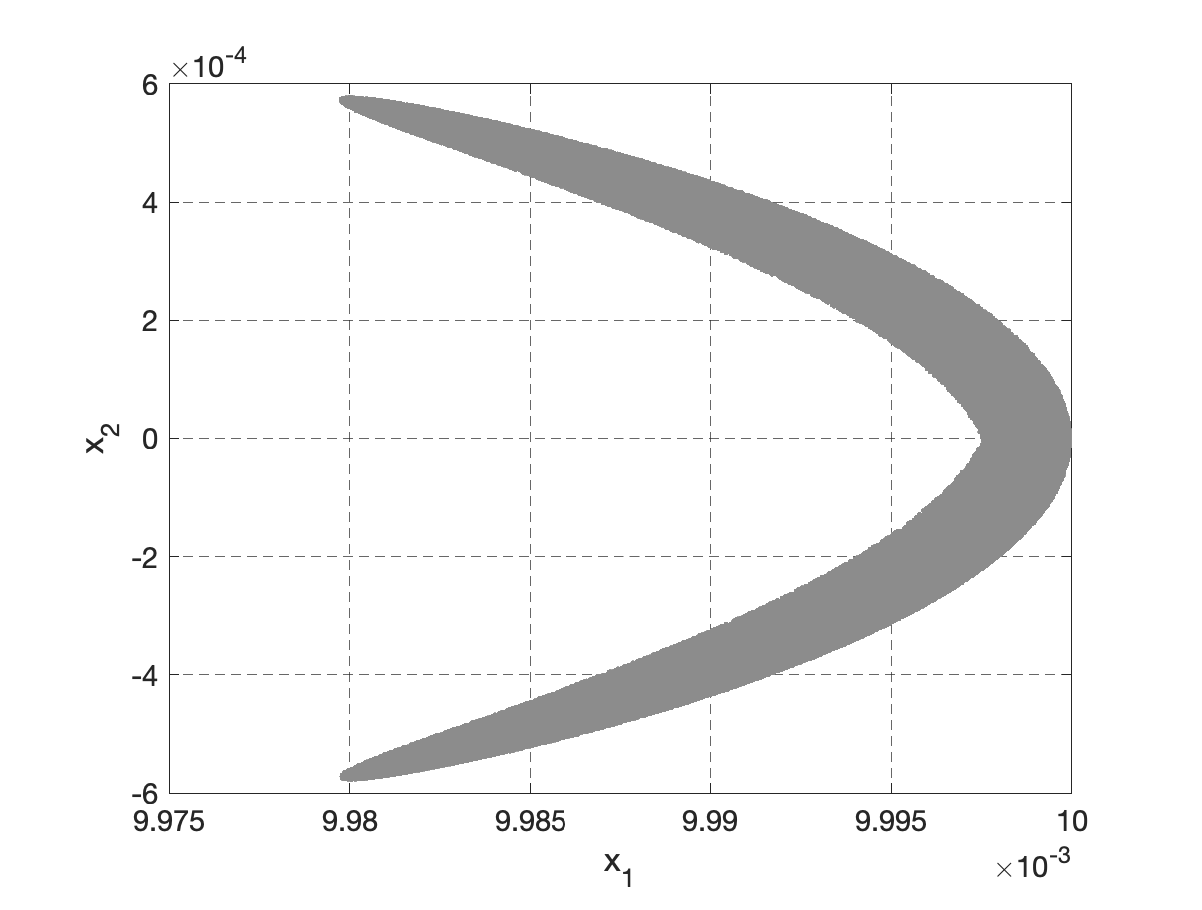
\includegraphics[width=\linewidth]{images/OsipovI_u=0_x1-x2.eps}
			%% This file was created by matlab2tikz.
%
%The latest updates can be retrieved from
%  http://www.mathworks.com/matlabcentral/fileexchange/22022-matlab2tikz-matlab2tikz
%where you can also make suggestions and rate matlab2tikz.
%
\begin{tikzpicture}
\node at (2.97,2.35) 
{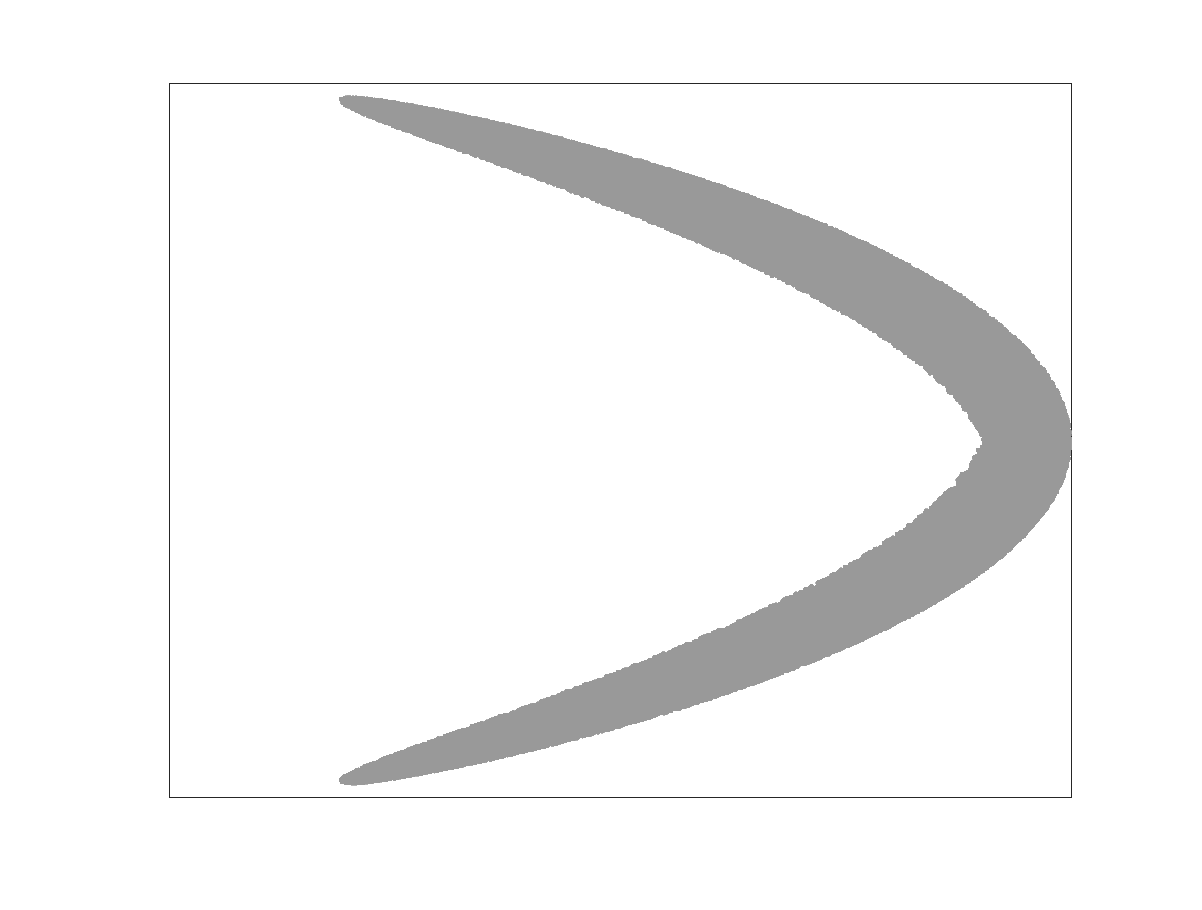
\includegraphics[width=0.985\linewidth]{images/OsipovI_u=0_x1-x2_1.eps}};
\pgfkeys{/pgf/number format/relative*={-3}}
\begin{axis}[%
width=0.761\linewidth,
height=0.6\linewidth,
at={(0\linewidth,0\linewidth)},
scale only axis,
xmin=0.009975,
xmax=0.01,
xlabel style={font=\color{white!15!black}},
xlabel={$ x_1 $},
ymin=-0.0006,
ymax=0.0006,
ylabel style={font=\color{white!15!black}},
ylabel={$ x_2 $},
xmajorgrids,
ymajorgrids,
grid style={dashed, opacity=0.7}
]
\end{axis}
\end{tikzpicture}%
			\subcaption{$ G_{x_1, x_2}(\varepsilon) $ системы \eqref{unicycle0};}
			\label{fig:u=0_x1-x2} 
		\end{minipage}
		\hfill
		\begin{minipage}[b]{.49\linewidth} 
			\small
			\centering
			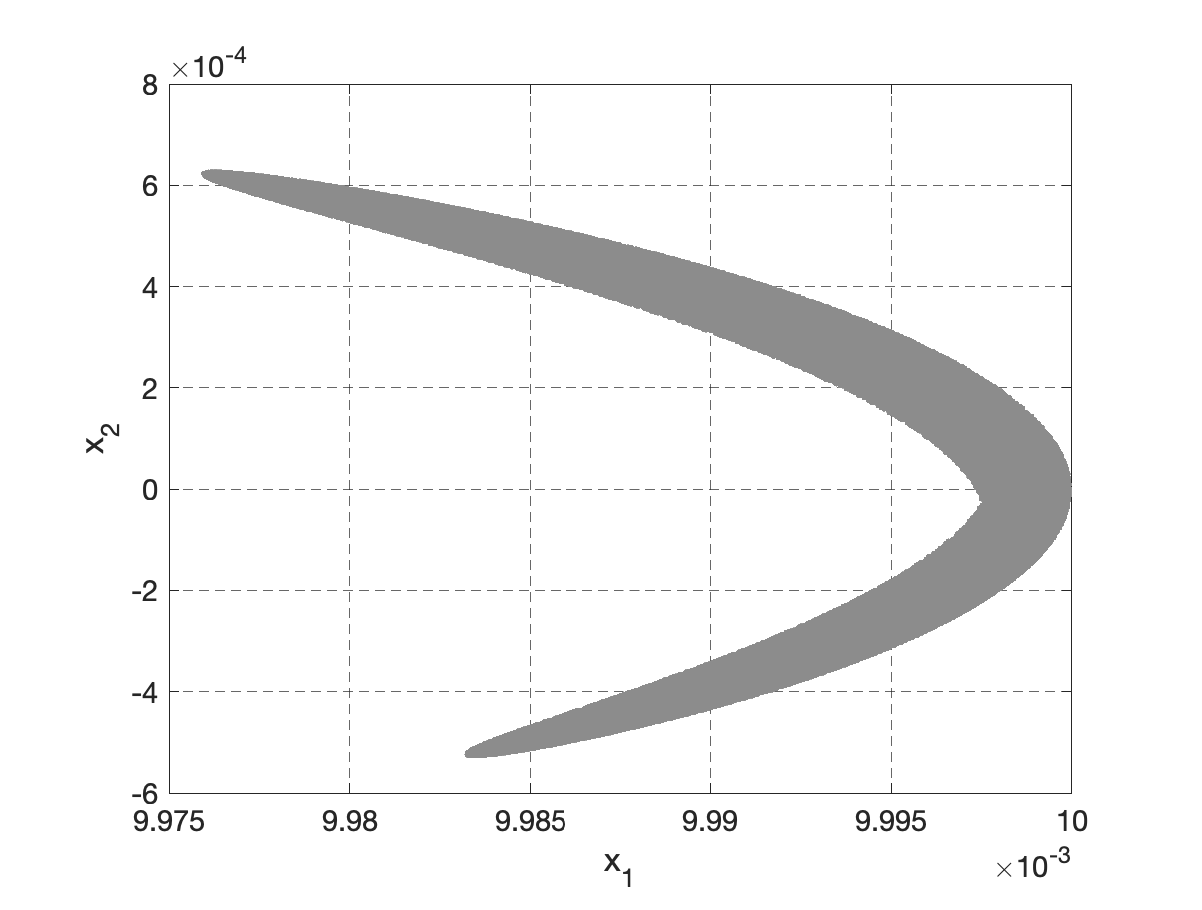
\includegraphics[width=\linewidth]{images/OsipovI_u=1_x1-x2.eps}
			%% This file was created by matlab2tikz.
%
%The latest updates can be retrieved from
%  http://www.mathworks.com/matlabcentral/fileexchange/22022-matlab2tikz-matlab2tikz
%where you can also make suggestions and rate matlab2tikz.
%
\begin{tikzpicture}
\node at (2.97,2.35) 
{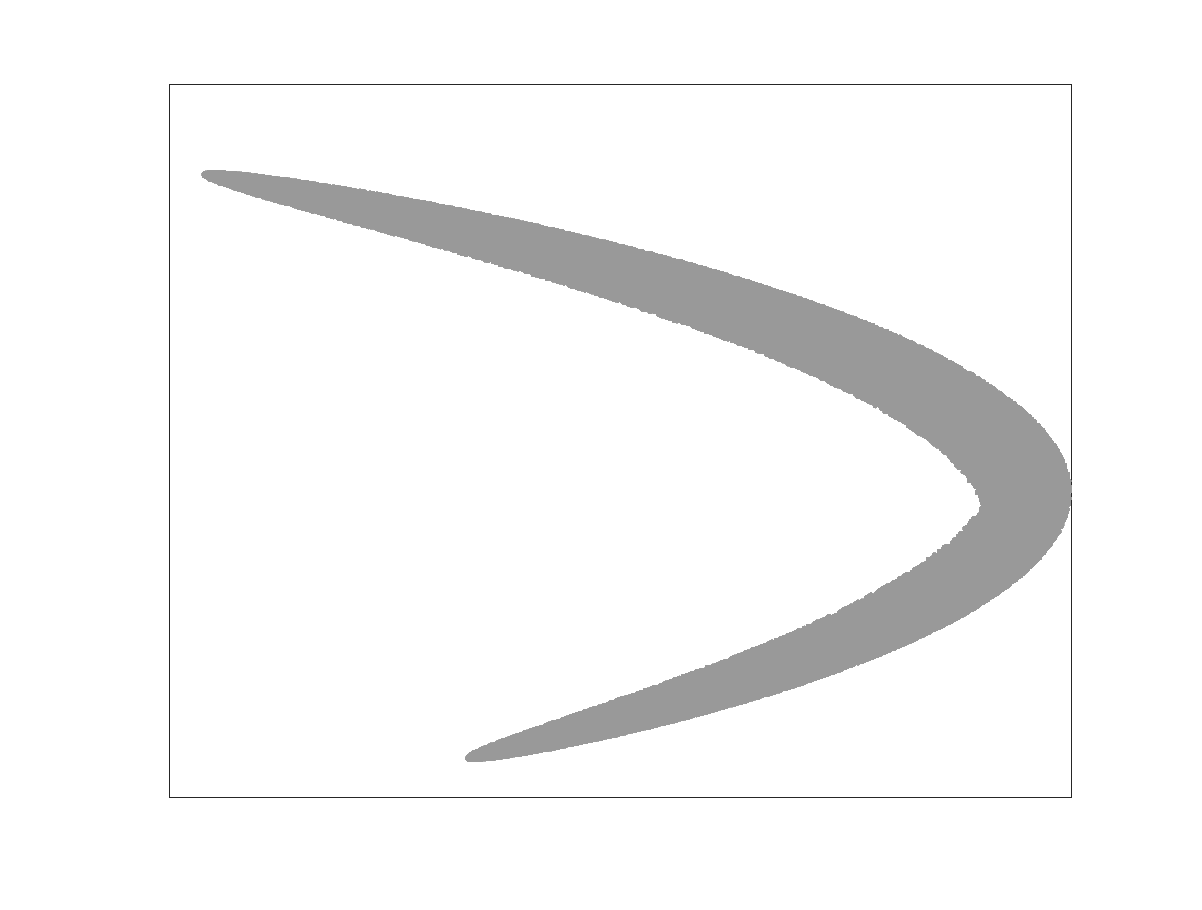
\includegraphics[width=0.985\linewidth]{OsipovI_u=1_x1-x2_1}};
\pgfkeys{/pgf/number format/relative*={-3}}
\begin{axis}[%
width=0.761\linewidth,
height=0.6\linewidth,
at={(0\linewidth,0\linewidth)},
scale only axis,
xmin=0.009975,
xmax=0.01,
xlabel style={font=\color{white!15!black}},
xlabel={$ x_1 $},
ymin=-0.0006,
ymax=0.0008,
ylabel style={font=\color{white!15!black}},
ylabel={$ x_2 $},
xmajorgrids,
ymajorgrids,
grid style={dashed, opacity=0.9}
]
\end{axis}
\end{tikzpicture}%
			\subcaption{$ G_{x_1, x_2}(\varepsilon) $ системы \eqref{unicycle1};}
			\label{fig:u=1_x1-x2}  
		\end{minipage} 
		\vfill
		\hspace{-2.5ex}
		\begin{minipage}[b]{.49\linewidth} 
			\small
			\centering 
			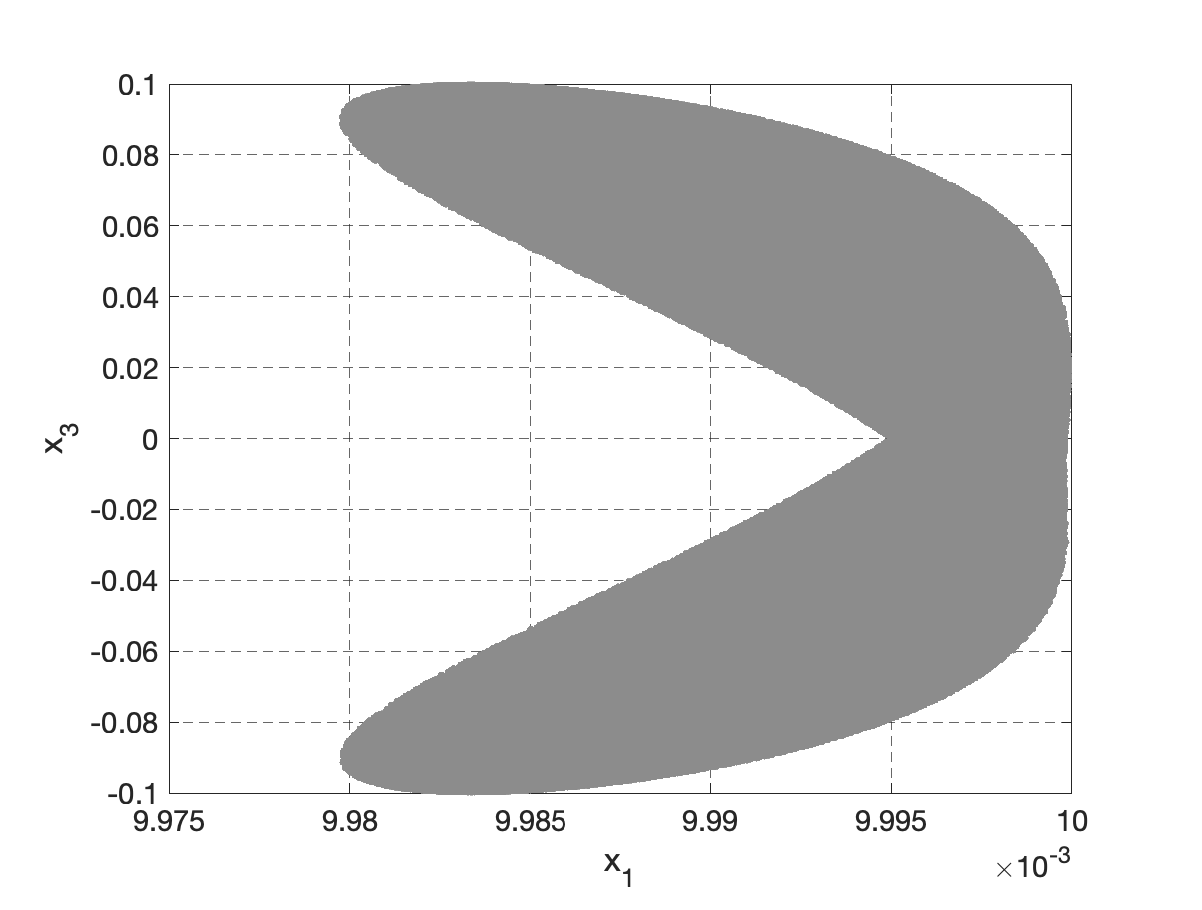
\includegraphics[width=\linewidth]{images/OsipovI_u=0_x1-x3.eps}
			%% This file was created by matlab2tikz.
%
%The latest updates can be retrieved from
%  http://www.mathworks.com/matlabcentral/fileexchange/22022-matlab2tikz-matlab2tikz
%where you can also make suggestions and rate matlab2tikz.
%
\begin{tikzpicture}
\node at (2.97,2.35) 
{
\includegraphics[width=0.985\linewidth]{OsipovI_u=0_x1-x3_1}};
\pgfkeys{/pgf/number format/.cd,fixed relative,precision=3}
\begin{axis}[%
width=0.761\linewidth,
height=0.6\linewidth,
at={(0\linewidth,0\linewidth)},
scale only axis,
xmin=0.009975,
xmax=0.01,
xlabel style={font=\color{white!15!black}},
ylabel near ticks,
xlabel={$ x_1 $},
ymin=-0.1,
ymax=0.1,
ylabel style={font=\color{white!15!black}},
ylabel={$ x_3 $},
xmajorgrids,
ymajorgrids,
grid style={dashed, opacity=0.7}
]
\end{axis}
\end{tikzpicture}%
			\subcaption{$ G_{x_1, x_3}(\varepsilon) $ системы \eqref{unicycle0};}
			\label{fig:u=0_x1-x3} 
		\end{minipage}
		\hfill
		\begin{minipage}[b]{.49\linewidth} 
			\small
			\centering
			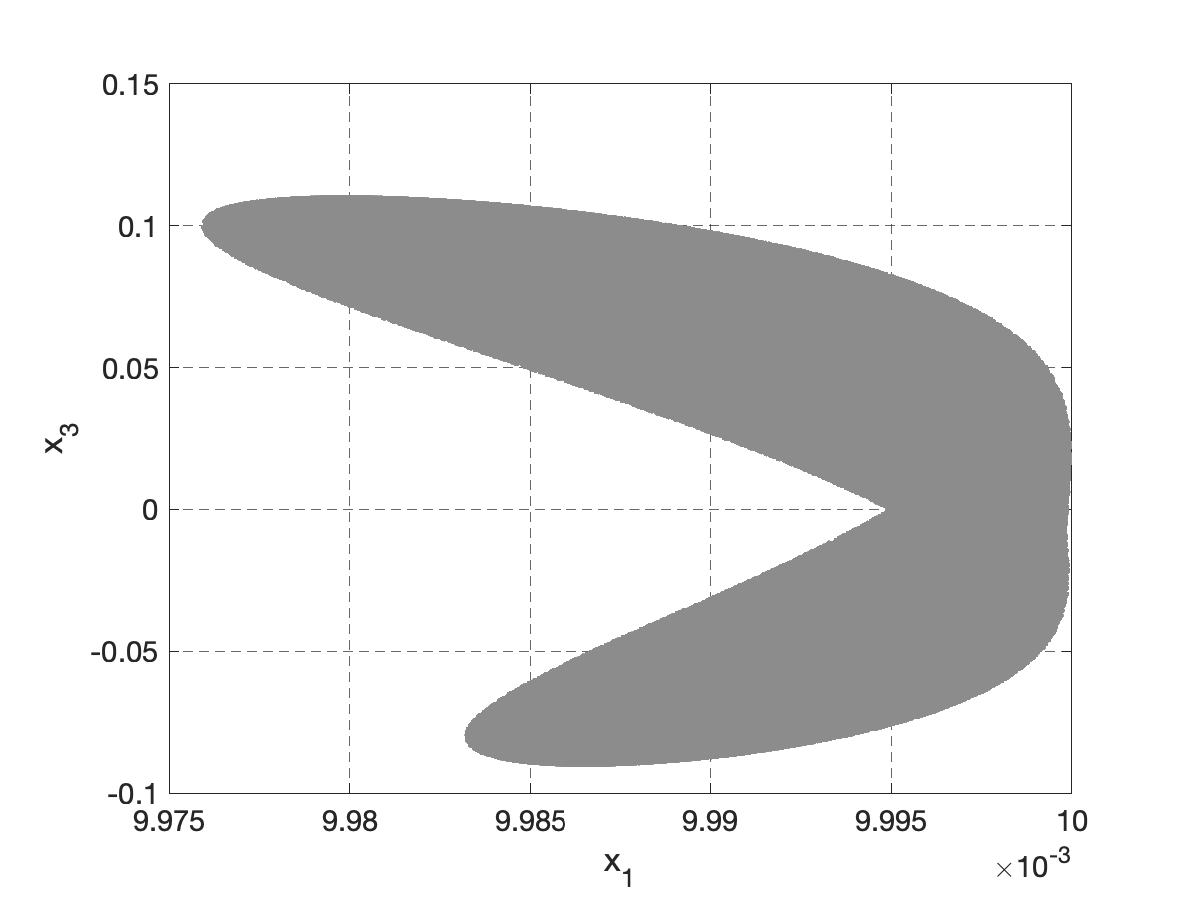
\includegraphics[width=\linewidth]{images/OsipovI_u=1_x1-x3.eps}
			%% This file was created by matlab2tikz.
%
%The latest updates can be retrieved from
%  http://www.mathworks.com/matlabcentral/fileexchange/22022-matlab2tikz-matlab2tikz
%where you can also make suggestions and rate matlab2tikz.
%
\begin{tikzpicture}
	
\node at (2.97,2.35) 
{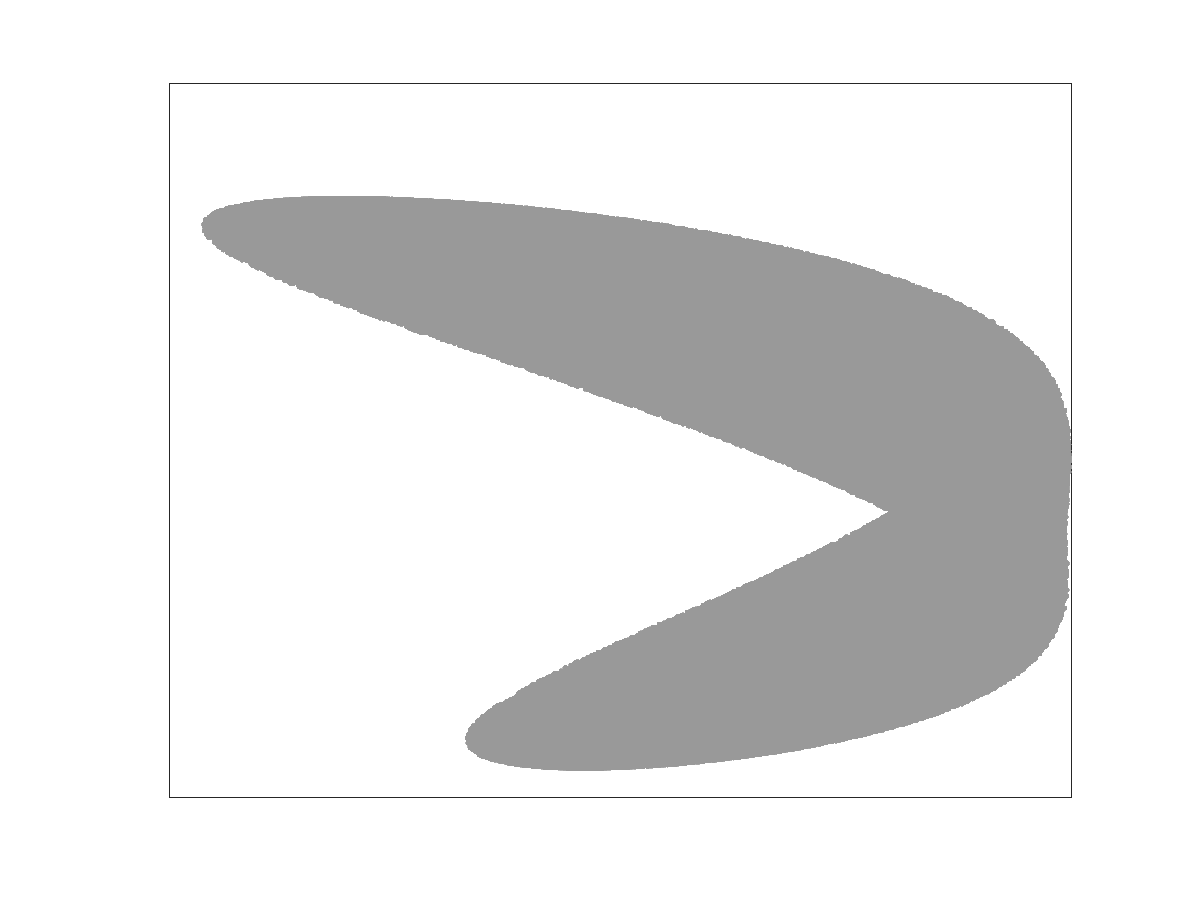
\includegraphics[width=0.985\linewidth]{OsipovI_u=1_x1-x3_1}};
\pgfkeys{/pgf/number format/relative*={-3}}

\begin{axis}[%
width=0.761\linewidth,
height=0.6\linewidth,
at={(0\linewidth,0\linewidth)},
scale only axis,
xmin=0.009975,
xmax=0.01,
xlabel style={font=\color{white!15!black}},
xlabel={$ x_1 $},
ymin=-0.1,
ymax=0.15,
ylabel style={font=\color{white!15!black}},
ylabel={$ x_3 $},
xmajorgrids,
ymajorgrids,
grid style={dashed, opacity=0.9}
]
\end{axis}
\end{tikzpicture}%
			\subcaption{$ G_{x_1, x_3}(\varepsilon) $ системы \eqref{unicycle1};}
			\label{fig:u=1_x1-x3}  
		\end{minipage} 
		\vfill
		\hspace{-2.5ex}
		\begin{minipage}[b]{.49\linewidth} 
			\small
			\centering 
			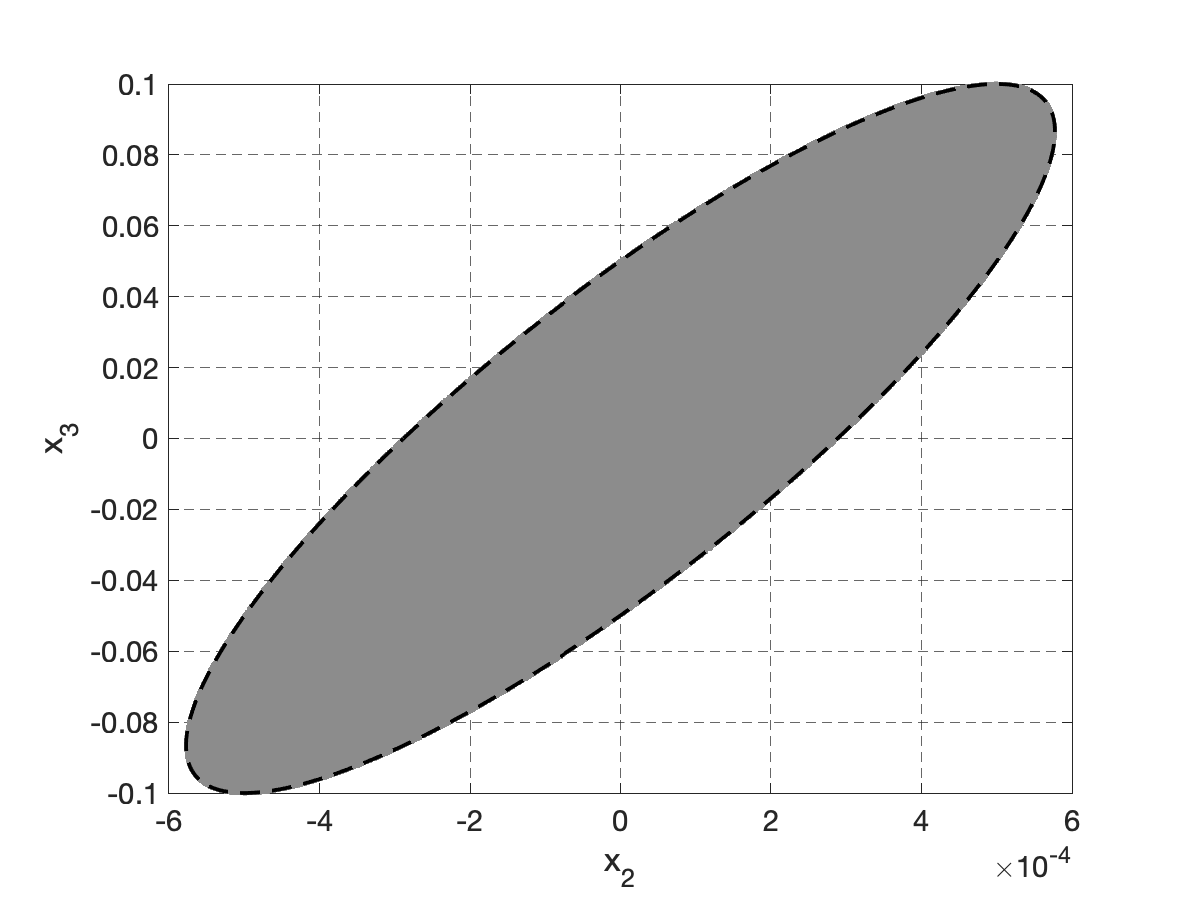
\includegraphics[width=\linewidth]{images/OsipovI_u=0_x2-x3.eps}
			%% This file was created by matlab2tikz.
%
%The latest updates can be retrieved from
%  http://www.mathworks.com/matlabcentral/fileexchange/22022-matlab2tikz-matlab2tikz
%where you can also make suggestions and rate matlab2tikz.
%
\begin{tikzpicture}
\node at (2.97,2.35) 
{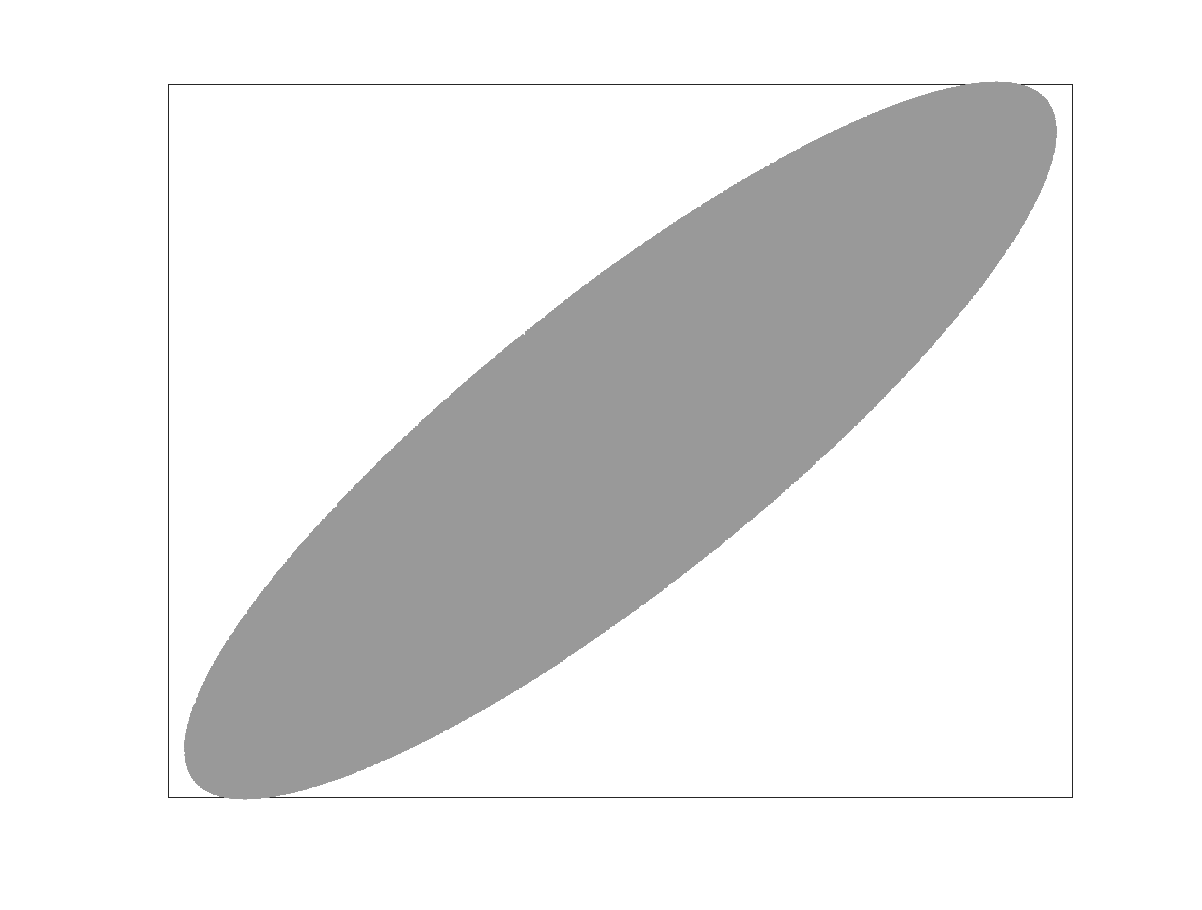
\includegraphics[width=0.985\linewidth]{OsipovI_u=0_x2-x3_1}};
\pgfkeys{/pgf/number format/.cd,fixed relative,precision=3}
\begin{axis}[%
width=0.761\linewidth,
height=0.6\linewidth,
at={(0\linewidth,0\linewidth)},
scale only axis,
xmin=-0.0006,
xmax=0.0006,
xlabel style={font=\color{white!15!black}},
xlabel={$ x_2 $},
ymin=-0.1,
ymax=0.1,
ylabel style={font=\color{white!15!black}},
ylabel={$ x_3 $},
xmajorgrids,
ymajorgrids,
grid style={dashed, opacity=0.7}
]
\addplot [color=black, dashed, line width=1.8pt, forget plot]
  table[row sep=crcr]{%
-0.00028866791780666	1.44335161666275e-06\\
-0.000279897676349703	0.00174668377533378\\
-0.0002710421753491	0.00349139214225243\\
-0.000262104112276241	0.00523503699730267\\
-0.000253086209751723	0.00697708720937059\\
-0.000243991214716013	0.00871701213308598\\
-0.000234821897592705	0.010454281770462\\
-0.00022558105144462	0.0121883669323379\\
-0.000216271491123012	0.0139187393995748\\
-0.000206896052410138	0.0156448720839568\\
-0.000197457591155454	0.0173662391887467\\
-0.000187958982405689	0.0190823163688491\\
-0.000178403119529083	0.0207925808905311\\
-0.00016879291333404	0.0224965117906516\\
-0.000159131291182461	0.024193590035352\\
-0.000149421196098048	0.0258832986781591\\
-0.000139665585869829	0.0275651230174517\\
-0.000129867432151182	0.0292385507532438\\
-0.000120029719554648	0.0309030721432363\\
-0.000110155444742784	0.0325581801580891\\
-0.000100247615515351	0.0342033706358677\\
-9.03092498931122e-05	0.035838142435615\\
-8.03433751985104e-05	0.0374619975900046\\
-7.03530271335194e-05	0.0390744414570258\\
-6.03412488549384e-05	0.0406749828706565\\
-5.03110900474174e-05	0.0422631342904774\\
-4.02656059944935e-05	0.0438384119501813\\
-3.02078566479219e-05	0.0454003360049329\\
-2.01409056955853e-05	0.0469484306775345\\
-1.00678196282645e-05	0.048482224403352\\
8.33319444416662e-09	0.0500012499739585\\
1.00844834787811e-05	0.0515050446794498\\
2.01575619317598e-05	0.0529931504493913\\
3.02245001961034e-05	0.0544651139923497\\
4.02822317848961e-05	0.0559204869339706\\
5.03276930156642e-05	0.0573588259535575\\
6.03578239436045e-05	0.0587796929191115\\
7.03695692936722e-05	0.0601826550207907\\
8.03598793912477e-05	0.0615672849027481\\
9.0325711091097e-05	0.0629331607933084\\
0.000100264028704343	0.0642798666334439\\
0.000110171804923167	0.0656069922035097\\
0.000120046021742952	0.0669141332482012\\
0.000129883671381603	0.0682008915996935\\
0.000139681757195739	0.0694668752989277\\
0.000149437294593506	0.0707116987150051\\
0.000159147311943709	0.0719349826626543\\
0.000168808851480998	0.0731363545177346\\
0.000178418970206839	0.074315448330741\\
0.000187974740785971	0.075471904938276\\
0.000197473252438107	0.076605372072454\\
0.000206911611824585	0.0777155044682059\\
0.000216286943929703	0.0788019639684498\\
0.000225596392936481	0.079864419627097\\
0.00023483712309657	0.0809025478098619\\
0.000244006319594044	0.0819160322928433\\
0.000253101189402829	0.0829045643588499\\
0.000262118962137475	0.0838678428914382\\
0.00027105689089705	0.0848055744666358\\
0.000279912253101871	0.0857174734423208\\
0.000288682351322827	0.0866032620452314\\
0.000297364514103041	0.0874626704555784\\
0.000305956096771624	0.0882954368892348\\
0.000314454482249267	0.0891013076774775\\
0.000322857081845429	0.089880037344258\\
0.000331161336046873	0.0906313886809759\\
0.000339364715297326	0.0913551328187356\\
0.000347464720767999	0.0920510492980618\\
0.00035545888511876	0.0927189261360531\\
0.000363344773249706	0.0933585598909551\\
0.000371119983042921	0.0939697557241295\\
0.00037878214609418	0.0945523274594049\\
0.000386328928434395	0.0951060976397873\\
0.000393758031240555	0.0956308975815151\\
0.000401067191535981	0.0961265674254422\\
0.000408254182879639	0.0965929561857326\\
0.000415316816044345	0.0970299217958519\\
0.00042225293968362	0.0974373311518421\\
0.000429060440987011	0.0978150601528669\\
0.000435737246323675	0.0981629937390134\\
0.000442281321874028	0.0984810259263407\\
0.000448690674249263	0.0987690598391637\\
0.000454963351098557	0.0990270077395624\\
0.000461097441703777	0.0992547910541074\\
0.000467091077561503	0.0994523403977945\\
0.000472942432952192	0.0996195955951801\\
0.000478649725496306	0.0997565056987106\\
0.000484211216697251	0.0998630290042424\\
0.00048962521247093	0.0999391330637446\\
0.000494890063661785	0.0999847946951835\\
0.00050000416654514	0.0999999999895837\\
0.000504965963315717	0.0999847443152654\\
0.000509773942562153	0.0999390323192546\\
0.000514426639727393	0.0998628779258683\\
0.00051892263755481	0.0997563043324723\\
0.000523260566519911	0.0996193440024157\\
0.00052743910524751	0.0994520386551416\\
0.000531456980914235	0.0992544392534797\\
0.000535312969636233	0.0990266059881218\\
0.000539005896841987	0.0987686082592877\\
0.000542534637630095	0.0984805246555848\\
0.000545898117111931	0.0981624429300695\\
0.00054909531073906	0.0978144599735168\\
0.000552125244615333	0.0974366817849062\\
0.000554986995793538	0.0970292234391336\\
0.000557679692556545	0.0965922090519583\\
0.000560202514682834	0.096125771742196\\
0.000562554693696348	0.0956300535911697\\
0.000564735513100572	0.0951052055994304\\
0.000566744308596789	0.0945513876407608\\
0.000568580468286433	0.0939687684134759\\
0.000570243432857474	0.0933575253890364\\
0.000571732695754795	0.0927178447579887\\
0.000573047803334489	0.0920499213732498\\
0.00057418835500205	0.091353958690753\\
0.000575154003334389	0.0906301687074733\\
0.00057594445418567	0.0898787718968512\\
0.000576559466776908	0.089099997141634\\
0.000576998853769308	0.0882940816641565\\
0.000577262481321336	0.0874612709540801\\
0.000577350269129487	0.0866018186936147\\
0.000577262190452743	0.0857159866802446\\
0.000576998272120724	0.0848040447469823\\
0.000576558594525508	0.0838662706801749\\
0.000575943291597151	0.0829029501348874\\
0.000575152550762886	0.08191437654789\\
0.000574186612890031	0.0809008510482736\\
0.000573045772212619	0.0798626823657238\\
0.000571730376241771	0.0788001867364783\\
0.000570240825659844	0.0777136878069983\\
0.000568577574198374	0.0766035165353828\\
0.000566741128499869	0.0754700110905558\\
0.000564732047963478	0.0743135167492561\\
0.000562550944574595	0.0731343857908635\\
0.000560198482718441	0.0719329773900902\\
0.000557675378977687	0.0707096575075735\\
0.000554982401914173	0.0694647987784002\\
0.000552120371834802	0.0681987803985984\\
0.000549090160541659	0.0669119880096307\\
0.000545892691066459	0.0656048135809243\\
0.000542528937389379	0.064277655290473\\
0.000538999924142375	0.0629309174035487\\
0.000535306726297067	0.0615650101495577\\
0.000531450468837296	0.0601803495970816\\
0.000527432326416442	0.058777357527138\\
0.000523253522999609	0.0573564613047026\\
0.0005189153314908	0.0559180937485293\\
0.000514419073345173	0.0544626929993095\\
0.000509766118166516	0.0529907023862101\\
0.000504957883290049	0.0515025702918314\\
0.000499995833350696	0.0499987500156252\\
0.000494881479836936	0.0484796996358155\\
0.000489616380630393	0.0469458818698633\\
0.00048420213953129	0.0453977639335186\\
0.000478640405769914	0.0438358173985018\\
0.000472932873504246	0.0422605180488582\\
0.000467081281303906	0.0406723457360301\\
0.000461087411620562	0.039071784232689\\
0.000454953090244985	0.0374593210853737\\
0.00044868018575089	0.0358354474659793\\
0.000442270608925752	0.0342006580221409\\
0.000435726312188764	0.0325554507265598\\
0.000429049288996108	0.0309003267253156\\
0.00042224157323373	0.0292357901852127\\
0.000415305238597798	0.0275623481402059\\
0.000408242397963038	0.0258805103369532\\
0.000401055202739125	0.0241907890795417\\
0.000393745842215349	0.0224936990734351\\
0.000386316542893733	0.0207897572686894\\
0.000378769567810818	0.0190794827024848\\
0.000371107215848326	0.0173633963410218\\
0.000363331821032889	0.0156420209208305\\
0.000355445751825092	0.0139158807895389\\
0.000347451410398008	0.0121855017461527\\
0.00033935123190548	0.0104514108808911\\
0.000331147683740344	0.00871413641462997\\
0.000322843264782841	0.00697420753800126\\
0.000314440504639433	0.0052321542501958\\
0.000305941962872257	0.00348850719752072\\
0.000297350228219465	0.00174379751175934\\
0.00028866791780666	-1.44335161666275e-06\\
0.000279897676349703	-0.00174668377533378\\
0.0002710421753491	-0.00349139214225243\\
0.000262104112276241	-0.00523503699730267\\
0.000253086209751723	-0.00697708720937059\\
0.000243991214716013	-0.00871701213308598\\
0.000234821897592705	-0.010454281770462\\
0.00022558105144462	-0.0121883669323379\\
0.000216271491123012	-0.0139187393995748\\
0.000206896052410138	-0.0156448720839568\\
0.000197457591155454	-0.0173662391887467\\
0.000187958982405689	-0.0190823163688491\\
0.000178403119529083	-0.0207925808905311\\
0.00016879291333404	-0.0224965117906516\\
0.000159131291182461	-0.024193590035352\\
0.000149421196098048	-0.0258832986781591\\
0.000139665585869829	-0.0275651230174517\\
0.000129867432151182	-0.0292385507532438\\
0.000120029719554648	-0.0309030721432363\\
0.000110155444742784	-0.0325581801580891\\
0.000100247615515351	-0.0342033706358677\\
9.03092498931122e-05	-0.035838142435615\\
8.03433751985104e-05	-0.0374619975900046\\
7.03530271335194e-05	-0.0390744414570258\\
6.03412488549384e-05	-0.0406749828706565\\
5.03110900474174e-05	-0.0422631342904774\\
4.02656059944935e-05	-0.0438384119501813\\
3.02078566479219e-05	-0.0454003360049329\\
2.01409056955853e-05	-0.0469484306775345\\
1.00678196282645e-05	-0.048482224403352\\
-8.33319444416662e-09	-0.0500012499739585\\
-1.00844834787811e-05	-0.0515050446794498\\
-2.01575619317598e-05	-0.0529931504493913\\
-3.02245001961034e-05	-0.0544651139923497\\
-4.02822317848961e-05	-0.0559204869339706\\
-5.03276930156642e-05	-0.0573588259535575\\
-6.03578239436045e-05	-0.0587796929191115\\
-7.03695692936722e-05	-0.0601826550207907\\
-8.03598793912477e-05	-0.0615672849027481\\
-9.0325711091097e-05	-0.0629331607933084\\
-0.000100264028704343	-0.0642798666334439\\
-0.000110171804923167	-0.0656069922035097\\
-0.000120046021742952	-0.0669141332482012\\
-0.000129883671381603	-0.0682008915996935\\
-0.000139681757195739	-0.0694668752989277\\
-0.000149437294593506	-0.0707116987150051\\
-0.000159147311943709	-0.0719349826626543\\
-0.000168808851480998	-0.0731363545177346\\
-0.000178418970206839	-0.074315448330741\\
-0.000187974740785971	-0.075471904938276\\
-0.000197473252438107	-0.076605372072454\\
-0.000206911611824585	-0.0777155044682059\\
-0.000216286943929703	-0.0788019639684498\\
-0.000225596392936481	-0.079864419627097\\
-0.00023483712309657	-0.0809025478098619\\
-0.000244006319594044	-0.0819160322928433\\
-0.000253101189402829	-0.0829045643588499\\
-0.000262118962137475	-0.0838678428914382\\
-0.00027105689089705	-0.0848055744666358\\
-0.000279912253101871	-0.0857174734423208\\
-0.000288682351322827	-0.0866032620452314\\
-0.000297364514103041	-0.0874626704555784\\
-0.000305956096771624	-0.0882954368892348\\
-0.000314454482249267	-0.0891013076774775\\
-0.000322857081845429	-0.089880037344258\\
-0.000331161336046873	-0.0906313886809759\\
-0.000339364715297326	-0.0913551328187356\\
-0.000347464720767999	-0.0920510492980618\\
-0.00035545888511876	-0.0927189261360531\\
-0.000363344773249706	-0.0933585598909551\\
-0.000371119983042921	-0.0939697557241295\\
-0.00037878214609418	-0.0945523274594049\\
-0.000386328928434395	-0.0951060976397873\\
-0.000393758031240555	-0.0956308975815151\\
-0.000401067191535981	-0.0961265674254422\\
-0.000408254182879639	-0.0965929561857326\\
-0.000415316816044345	-0.0970299217958519\\
-0.00042225293968362	-0.0974373311518421\\
-0.000429060440987011	-0.0978150601528669\\
-0.000435737246323675	-0.0981629937390134\\
-0.000442281321874028	-0.0984810259263407\\
-0.000448690674249263	-0.0987690598391637\\
-0.000454963351098557	-0.0990270077395624\\
-0.000461097441703777	-0.0992547910541074\\
-0.000467091077561503	-0.0994523403977945\\
-0.000472942432952192	-0.0996195955951801\\
-0.000478649725496306	-0.0997565056987106\\
-0.000484211216697251	-0.0998630290042424\\
-0.00048962521247093	-0.0999391330637446\\
-0.000494890063661785	-0.0999847946951835\\
-0.00050000416654514	-0.0999999999895837\\
-0.000504965963315717	-0.0999847443152654\\
-0.000509773942562153	-0.0999390323192546\\
-0.000514426639727393	-0.0998628779258683\\
-0.00051892263755481	-0.0997563043324723\\
-0.000523260566519911	-0.0996193440024157\\
-0.00052743910524751	-0.0994520386551416\\
-0.000531456980914235	-0.0992544392534797\\
-0.000535312969636233	-0.0990266059881218\\
-0.000539005896841987	-0.0987686082592877\\
-0.000542534637630095	-0.0984805246555848\\
-0.000545898117111931	-0.0981624429300695\\
-0.00054909531073906	-0.0978144599735168\\
-0.000552125244615333	-0.0974366817849062\\
-0.000554986995793538	-0.0970292234391336\\
-0.000557679692556545	-0.0965922090519583\\
-0.000560202514682834	-0.096125771742196\\
-0.000562554693696348	-0.0956300535911697\\
-0.000564735513100572	-0.0951052055994304\\
-0.000566744308596789	-0.0945513876407608\\
-0.000568580468286433	-0.0939687684134759\\
-0.000570243432857474	-0.0933575253890364\\
-0.000571732695754795	-0.0927178447579887\\
-0.000573047803334489	-0.0920499213732498\\
-0.00057418835500205	-0.091353958690753\\
-0.000575154003334389	-0.0906301687074733\\
-0.00057594445418567	-0.0898787718968512\\
-0.000576559466776908	-0.089099997141634\\
-0.000576998853769308	-0.0882940816641565\\
-0.000577262481321336	-0.0874612709540801\\
-0.000577350269129487	-0.0866018186936147\\
-0.000577262190452743	-0.0857159866802446\\
-0.000576998272120724	-0.0848040447469823\\
-0.000576558594525508	-0.0838662706801749\\
-0.000575943291597151	-0.0829029501348874\\
-0.000575152550762886	-0.08191437654789\\
-0.000574186612890031	-0.0809008510482736\\
-0.000573045772212619	-0.0798626823657238\\
-0.000571730376241771	-0.0788001867364783\\
-0.000570240825659844	-0.0777136878069983\\
-0.000568577574198374	-0.0766035165353828\\
-0.000566741128499869	-0.0754700110905558\\
-0.000564732047963478	-0.0743135167492561\\
-0.000562550944574595	-0.0731343857908635\\
-0.000560198482718441	-0.0719329773900902\\
-0.000557675378977687	-0.0707096575075735\\
-0.000554982401914173	-0.0694647987784002\\
-0.000552120371834802	-0.0681987803985984\\
-0.000549090160541659	-0.0669119880096307\\
-0.000545892691066459	-0.0656048135809243\\
-0.000542528937389379	-0.064277655290473\\
-0.000538999924142375	-0.0629309174035487\\
-0.000535306726297067	-0.0615650101495577\\
-0.000531450468837296	-0.0601803495970816\\
-0.000527432326416442	-0.058777357527138\\
-0.000523253522999609	-0.0573564613047026\\
-0.0005189153314908	-0.0559180937485293\\
-0.000514419073345173	-0.0544626929993095\\
-0.000509766118166516	-0.0529907023862101\\
-0.000504957883290049	-0.0515025702918314\\
-0.000499995833350696	-0.0499987500156252\\
-0.000494881479836936	-0.0484796996358155\\
-0.000489616380630393	-0.0469458818698633\\
-0.00048420213953129	-0.0453977639335186\\
-0.000478640405769914	-0.0438358173985018\\
-0.000472932873504246	-0.0422605180488582\\
-0.000467081281303906	-0.0406723457360301\\
-0.000461087411620562	-0.039071784232689\\
-0.000454953090244985	-0.0374593210853737\\
-0.00044868018575089	-0.0358354474659793\\
-0.000442270608925752	-0.0342006580221409\\
-0.000435726312188764	-0.0325554507265598\\
-0.000429049288996108	-0.0309003267253156\\
-0.00042224157323373	-0.0292357901852127\\
-0.000415305238597798	-0.0275623481402059\\
-0.000408242397963038	-0.0258805103369532\\
-0.000401055202739125	-0.0241907890795417\\
-0.000393745842215349	-0.0224936990734351\\
-0.000386316542893733	-0.0207897572686894\\
-0.000378769567810818	-0.0190794827024848\\
-0.000371107215848326	-0.0173633963410218\\
-0.000363331821032889	-0.0156420209208305\\
-0.000355445751825092	-0.0139158807895389\\
-0.000347451410398008	-0.0121855017461527\\
-0.00033935123190548	-0.0104514108808911\\
-0.000331147683740344	-0.00871413641462997\\
-0.000322843264782841	-0.00697420753800126\\
-0.000314440504639433	-0.0052321542501958\\
-0.000305941962872257	-0.00348850719752072\\
-0.000297350228219465	-0.00174379751175934\\
-0.00028866791780666	1.44335161666275e-06\\
};
\end{axis}
\end{tikzpicture}%
			\subcaption{$ G_{x_2, x_3}(\varepsilon) $ системы \eqref{unicycle0};}
			\label{fig:u=0_x2-x3} 
		\end{minipage}
		\hfill
		\begin{minipage}[b]{.49\linewidth} 
			\small
			\centering
			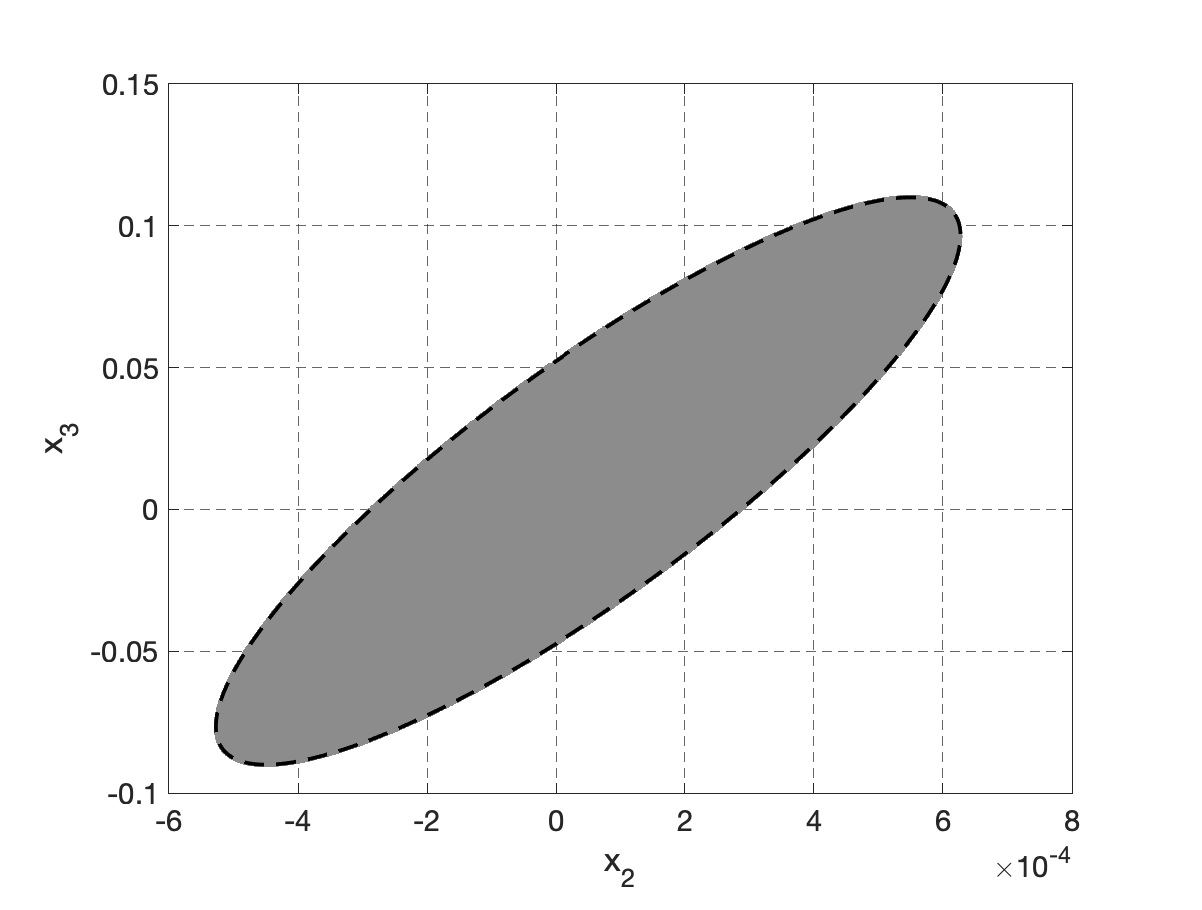
\includegraphics[width=\linewidth]{images/OsipovI_u=1_x2-x3.eps}
			%% This file was created by matlab2tikz.
%
%The latest updates can be retrieved from
%  http://www.mathworks.com/matlabcentral/fileexchange/22022-matlab2tikz-matlab2tikz
%where you can also make suggestions and rate matlab2tikz.
%
\begin{tikzpicture}
\node at (2.97,2.35) 
{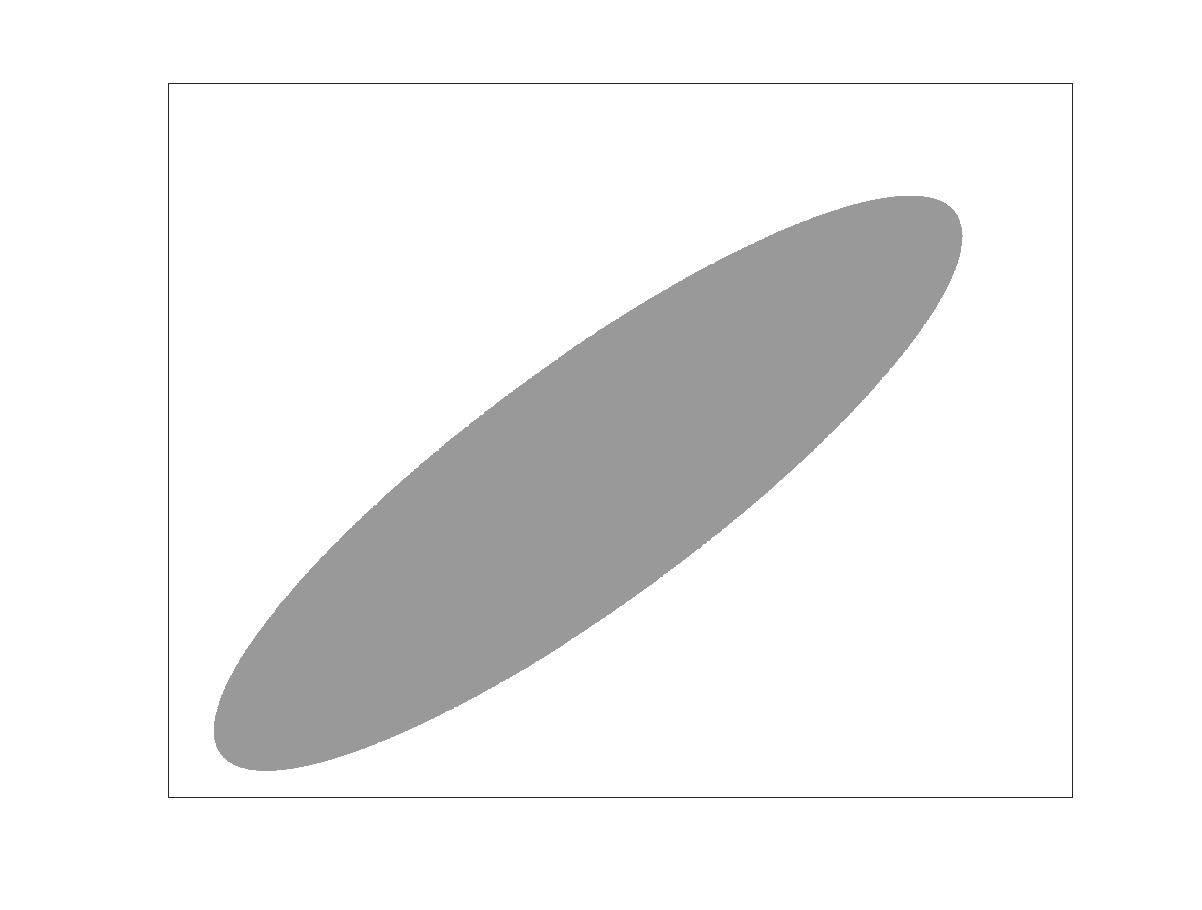
\includegraphics[width=0.985\linewidth]{OsipovI_u=1_x2-x3_1}};
\begin{axis}[%
width=0.761\linewidth,
height=0.6\linewidth,
at={(0\linewidth,0\linewidth)},
scale only axis,
xmin=-0.0006,
xmax=0.0008,
xlabel style={font=\color{white!15!black}},
xlabel={$ x_2 $},
ymin=-0.1,
ymax=0.15,
ylabel style={font=\color{white!15!black}},
ylabel={$ x_3 $},
xmajorgrids,
ymajorgrids,
grid style={dashed, opacity=0.9}
]
\addplot [color=black, dashed, line width=1.8pt, forget plot]
  table[row sep=crcr]{%
-0.000238655344918043	0.0100014432505853\\
-0.000212092211410247	0.0152350368964098\\
-0.000184810702510835	0.0204542816699843\\
-0.000156885594939385	0.0256448719841695\\
-0.000128393429474696	0.0307925807917078\\
-9.94123011618386e-05	0.0358832985805707\\
-7.00216452590718e-05	0.0409030720471502\\
-4.03020195113013e-05	0.0458381423412946\\
-1.03348833469241e-05	0.0506749827783604\\
1.97976253968335e-05	0.055400335914914\\
5.00129156079804e-05	0.0600012498864635\\
7.01615368250419e-05	0.0629931503637126\\
9.02855938074709e-05	0.0659204868502126\\
0.00011036056849173	0.0687796928373763\\
0.00013036200261346	0.0715672848231352\\
0.000150265527506188	0.0742798665560503\\
0.000170046893790729	0.0769141331731213\\
0.000189682000919345	0.0794668752262528\\
0.000209146926538575	0.081934982592473\\
0.000228417955634871	0.084315448263139\\
0.000247471609427757	0.0866053720075135\\
0.00026628467397509	0.0888019639062498\\
0.000284834228455641	0.0909025477504784\\
0.00030309767309461	0.0929045643023551\\
0.000321052756697984	0.0948055744130986\\
0.000338677603762161	0.096603261994717\\
0.000355950741125877	0.0982954368418047\\
0.00037285112413199	0.0998800372999701\\
0.000389358162267109	0.101355132777644\\
0.000405451744247984	0.102718926098207\\
0.00042111226252399	0.103969755689576\\
0.000436320637165935	0.105106097608568\\
0.000451058339111979	0.106126567397596\\
0.000458245053689743	0.106592956159585\\
0.000465307412742477	0.107029921771412\\
0.000472243265007194	0.107437331129116\\
0.000479050497756109	0.107815060131863\\
0.000485727037440181	0.108162993719737\\
0.000492270850320747	0.108481025908798\\
0.000498679943089012	0.10876905982336\\
0.000504952363473227	0.109027007725503\\
0.000511086200833386	0.109254791041796\\
0.000517079586743199	0.109452340387235\\
0.000522930695559282	0.109619595586376\\
0.00052863774497719	0.109756505691665\\
0.000534198996574392	0.109863028998956\\
0.000539612756339777	0.10993913306022\\
0.00054487737518967	0.109984794693422\\
0.00054999124947018	0.109999999989585\\
0.000554952821445659	0.10998474431703\\
0.000559760579773208	0.109939032322782\\
0.00056441305996309	0.109862877931157\\
0.000568908844824745	0.109756304339521\\
0.000573246564898572	0.109619344011223\\
0.000577424898872997	0.109452038665704\\
0.000581442573987026	0.109254439265794\\
0.000585298366417908	0.109026606002184\\
0.000588991101653905	0.108768608275094\\
0.000592519654852089	0.10848052467313\\
0.000595882951180973	0.108162442949349\\
0.000599079966147928	0.107814459994524\\
0.000602109725911223	0.107436681807635\\
0.000604971307576668	0.107029223463577\\
0.000607663839478786	0.106592209078109\\
0.000610186501446258	0.106125771770045\\
0.000612538525051817	0.10563005362071\\
0.000616727843576859	0.104551387673655\\
0.000620226691014594	0.103357525425244\\
0.000623030804558375	0.102049921412727\\
0.000625136767827786	0.100630168750172\\
0.000626542015030984	0.0990999971875026\\
0.000627244834090712	0.0974612710030624\\
0.000627244368730212	0.0957159867322809\\
0.000626540619516447	0.0938662707352017\\
0.000625134443859435	0.0919143766058404\\
0.000623027554967598	0.0898626824265272\\
0.00062022251976053	0.0877136878705805\\
0.000616722755741525	0.0854700111568394\\
0.000612532526833964	0.0831343858597678\\
0.000607656938186305	0.0807096575790145\\
0.00060210192995229	0.078198780472489\\
0.000595874270053767	0.0756048136571746\\
0.000588981545935036	0.0729309174820657\\
0.000581432155318667	0.0701803496777697\\
0.000573235295974264	0.0673564613874635\\
0.000564400954512281	0.0644626930840423\\
0.000554939894216983	0.0615025703784329\\
0.000544863641932958	0.0584796997241802\\
0.00053418447402151	0.0553977640235389\\
0.00051706391371599	0.0506723458283275\\
0.000498663162546154	0.0458354475603007\\
0.000479032655691922	0.0409003268214026\\
0.00045822619900808	0.0358805104345424\\
0.000436300821546165	0.0307897573675133\\
0.00041331661924178	0.0256420210206182\\
0.000389336590195827	0.0204514109813691\\
0.000364426462001091	0.0152321543510888\\
0.000338654511587488	0.0099985567494147\\
0.000312091378079693	0.00476496310359015\\
0.00028480986918028	-0.000454281669984291\\
0.00025688476160883	-0.00564487198416951\\
0.000228392596144142	-0.0107925807917078\\
0.000199411467831284	-0.0158832985805707\\
0.000170020811928517	-0.0209030720471502\\
0.000140301186180747	-0.0258381423412947\\
0.00011033405001637	-0.0306749827783604\\
8.0201541272612e-05	-0.035400335914914\\
4.99862510614513e-05	-0.0400012498864635\\
2.98376298444036e-05	-0.0429931503637126\\
9.71357286197461e-06	-0.0459204868502126\\
-1.03614018222842e-05	-0.0487796928373763\\
-3.03628359440145e-05	-0.0515672848231352\\
-5.02663608367426e-05	-0.0542798665560503\\
-7.00477271212835e-05	-0.0569141331731213\\
-8.96828342499129e-05	-0.0594668752262528\\
-0.00010914775986913	-0.0619349825924731\\
-0.000128418788965426	-0.064315448263139\\
-0.000147472442758312	-0.0666053720075135\\
-0.000166285507305644	-0.0688019639062498\\
-0.000184835061786195	-0.0709025477504784\\
-0.000203098506425164	-0.0729045643023551\\
-0.000221053590028539	-0.0748055744130986\\
-0.000238678437092715	-0.076603261994717\\
-0.000255951574456431	-0.0782954368418047\\
-0.000272851957462544	-0.0798800372999701\\
-0.000289358995597663	-0.0813551327776438\\
-0.000305452577578538	-0.0827189260982075\\
-0.000321113095854544	-0.0839697556895761\\
-0.00033632147049649	-0.0851060976085683\\
-0.000351059172442533	-0.0861265673975956\\
-0.000358245887020298	-0.0865929561595852\\
-0.000365308246073032	-0.0870299217714116\\
-0.000372244098337748	-0.0874373311291165\\
-0.000379051331086663	-0.0878150601318628\\
-0.000385727870770736	-0.0881629937197372\\
-0.000392271683651302	-0.0884810259087982\\
-0.000398680776419566	-0.0887690598233604\\
-0.000404953196803781	-0.089027007725503\\
-0.00041108703416394	-0.0892547910417962\\
-0.000417080420073754	-0.0894523403872353\\
-0.000422931528889836	-0.0896195955863761\\
-0.000428638578307744	-0.0897565056916645\\
-0.000434199829904947	-0.0898630289989563\\
-0.000439613589670332	-0.0899391330602201\\
-0.000444878208520225	-0.0899847946934217\\
-0.000449992082800735	-0.0899999999895852\\
-0.000454953654776213	-0.0899847443170301\\
-0.000459761413103763	-0.089939032322782\\
-0.000464413893293644	-0.0898628779311573\\
-0.000468909678155299	-0.0897563043395214\\
-0.000473247398229126	-0.0896193440112226\\
-0.000477425732203551	-0.0894520386657038\\
-0.000481443407317581	-0.0892544392657938\\
-0.000485299199748462	-0.0890266060021841\\
-0.000488991934984459	-0.0887686082750939\\
-0.000492520488182643	-0.0884805246731301\\
-0.000495883784511528	-0.0881624429493486\\
-0.000499080799478482	-0.0878144599945238\\
-0.000502110559241778	-0.0874366818076348\\
-0.000504972140907223	-0.0870292234635768\\
-0.000507664672809341	-0.0865922090781085\\
-0.000510187334776813	-0.0861257717700454\\
-0.000512539358382372	-0.0856300536207098\\
-0.000516728676907427	-0.0845513876736548\\
-0.000520227524345149	-0.0833575254252442\\
-0.000523031637888929	-0.0820499214127272\\
-0.00052513760115834	-0.0806301687501723\\
-0.000526542848361539	-0.0790999971875026\\
-0.000527245667421267	-0.0774612710030624\\
-0.000527245202060767	-0.0757159867322809\\
-0.000526541452847001	-0.0738662707352017\\
-0.000525135277189989	-0.0719143766058404\\
-0.000523028388298152	-0.0698626824265272\\
-0.000520223353091084	-0.0677136878705805\\
-0.000516723589072079	-0.0654700111568394\\
-0.000512533360164519	-0.0631343858597678\\
-0.000507657771516859	-0.0607096575790145\\
-0.000502102763282844	-0.058198780472489\\
-0.000495875103384322	-0.0556048136571746\\
-0.00048898237926559	-0.0529309174820657\\
-0.000481432988649222	-0.0501803496777697\\
-0.000473236129304819	-0.0473564613874635\\
-0.000464401787842836	-0.0444626930840423\\
-0.000454940727547537	-0.0415025703784329\\
-0.000444864475263512	-0.0384796997241802\\
-0.000434185307352064	-0.0353977640235389\\
-0.000417064747046544	-0.0306723458283275\\
-0.000398663995876708	-0.0258354475603007\\
-0.000379033489022476	-0.0209003268214026\\
-0.000358227032338634	-0.0158805104345424\\
-0.000336301654876719	-0.0107897573675133\\
-0.000313317452572334	-0.00564202102061818\\
-0.000289337423526381	-0.00045141098136911\\
-0.000264427295331646	0.00476784564891122\\
-0.000238655344918043	0.0100014432505853\\
};
\end{axis}
\end{tikzpicture}%
			\subcaption{$ G_{x_2, x_3}(\varepsilon) $ системы \eqref{unicycle1};}
			\label{fig:u=1_x2-x3}  
		\end{minipage}
		\caption{Результаты численного эксперимента для $ \varepsilon = 0.01 $.}\label{fig:RS}
	\end{figure}
	
	Немного изменим рассмотренный пример для того, чтобы линеаризованная система оставалась управляемой. Итак, рассматривается нелинейная система
	\begin{equation}\label{unicycle1}
		\dot{x_1} = \cos(x_3), \qquad
		\dot{x_2} = \sin(x_3), \qquad
		\dot{x_3} = 1 + u(t), \qquad 0 \leq t \leq \varepsilon
	\end{equation}
	при интегральных ограничениях на управление 
	\begin{equation*}
		\int_0^1 u^2(t) dt \leqslant 1
	\end{equation*}
	и нулевых начальных условиях $ x_1(0) = x_2(0) = x_3(0) = 0 $. Фактически, это то же самое, что рассматривать исходную систему при ограничении $ \displaystyle{\int_0^1} \left( u(t) - 1\right)^2 \ dt \leqslant 1$.
	
	Порождённое нулевым управлением $ u(t) \equiv 0 $ решение обозначим $ x(t,0) = x(t) $ и будем использовать его как опорное. 
	\begin{gather}\label{trj}
		\begin{gathered}
			\dot{x_3} = 1 \longrightarrow x_3(t) = x_3(0) + t = t, \\
			\dot{x_2} = \sin(x_3(t)) = \sin(t) \longrightarrow x_2(t) = x_2(0) + \int_0^t \sin(\tau) d\tau = 1 - \cos(t),\\
			\dot{x_1} = \cos(x_3(t)) = \cos(t) \longrightarrow x_1(t) = x_1(0) + \int_0^t \cos(\tau) d\tau = \sin(t).
		\end{gathered}
	\end{gather}
	Выпишем матрицы линеаризованной вдоль траектории \eqref{trj} системы 
	\begin{gather*}
		A(t) = \begin{pmatrix}
			0 & 0 & -\sin(t) \\ 
			0 & 0 & \cos(t) \\ 
			0 & 0 & 0
		\end{pmatrix}, \qquad  B = \begin{pmatrix}
			0 \\ 
			0 \\ 
			1
		\end{pmatrix}.
	\end{gather*}
	Для изучения грамиана управляемости выпишем фундаментальную матрицу линеаризованной системы
	\begin{gather*}
		\begin{gathered}
			X(t,\tau) = \begin{pmatrix}
				1 & 0 & \cos(t)-\cos(t_1) \\ 
				0 & 1 & \sin(t)-\sin(t_1) \\ 
				0 & 0 & 1
			\end{pmatrix}.
		\end{gathered}	
	\end{gather*}
	Грамиан управляемости имеет вид
	\begin{gather*}
		W(\varepsilon) = \int_0^{\varepsilon}X(\varepsilon,t) B B^{\top} X^{\top}(\varepsilon,t)dt =
	\end{gather*}
	\begin{gather*}
		=\begin{pmatrix}
			\varepsilon-\dfrac{3}{4} \sin(2\varepsilon) +\dfrac{1}{2}\varepsilon \cos(2\varepsilon)& \dfrac{3}{2}\cos^2(\varepsilon) - \cos(\varepsilon) + \dfrac{1}{2}\varepsilon \sin(2 \varepsilon) - \dfrac{1}{2} &  \varepsilon\cos( \varepsilon)-\sin( \varepsilon) \\[8pt] 
			* & \dfrac{3}{4}\sin(2\varepsilon) + \dfrac{1}{2}\varepsilon + \varepsilon \sin^2(\varepsilon) - 2 \sin(\varepsilon) & \cos(\varepsilon) + \varepsilon\sin(\varepsilon)-1 \\ 
			* & * & \varepsilon
		\end{pmatrix}.	
	\end{gather*}
	Здесь и далее, будем заменять элементы симметричных матриц под главной диагональю на $ * $ для лаконичной записи.
	Проделаем замену времени $ t = \varepsilon \tau $ и выпишем грамиан управляемости $ \widetilde{W}(\varepsilon) $ линеаризованной системы в новом времени $ \tau $
	\begin{gather*}
		\widetilde{W}(\varepsilon) = \dfrac{1}{\varepsilon} W(\varepsilon) = 
	\end{gather*} \footnotesize
	\begin{gather*}
		=\begin{pmatrix} 
			\cos^2(\varepsilon)-\dfrac{3}{4\varepsilon}\sin(2\varepsilon)+\dfrac{1}{2} & 
			\cos\left(\varepsilon \right)\,\sin\left(\varepsilon \right)+\dfrac{1}{2\,\varepsilon}\left( 3\cos^2\left(\varepsilon \right)-2\cos\left(\varepsilon\right)-1\right) &
			\cos\left(\varepsilon \right)-\dfrac{1}{\varepsilon} \sin\left(\varepsilon \right) \\[8pt] 
			* &
			\dfrac{3}{2}-\dfrac{2\,\sin\left(\varepsilon \right)-\dfrac{3\,\cos\left(\varepsilon \right)\,\sin\left(\varepsilon \right)}{2}}{\varepsilon }-{\cos\left(\varepsilon \right)}^2 & \sin\left(\varepsilon \right)+\dfrac{1}{\varepsilon } \left(\cos\left(\varepsilon \right)-1 \right)\\
			* &
			* & 
			1 \end{pmatrix}.	
	\end{gather*}
	\normalsize
	Далее последовательно рассмотрим проекции системы \eqref{unicycle1} на координатные плоскости $ (x_1, x_2) $, $ (x_1, x_3) $, $ (x_2, x_3) $. \\
	
	\begin{enumerate}
		\item Будем рассматривать проекцию $ G_{x_1, x_2}(\varepsilon) $ области достижимости системы \eqref{unicycle1} на плоскость первых двух фазовых координат. Матрица проектирования будет иметь вид
		\begin{equation*}
			C = \begin{pmatrix}
				1 & 0 & 0 \\ 
				0 & 1 & 0 
			\end{pmatrix}. 
		\end{equation*} 
		Тогда: \small
		\begin{equation}\label{Ve}
			\widetilde{W}_{x_1,x_2}(\varepsilon)= \begin{pmatrix}
				\cos^2(\varepsilon)-\dfrac{3}{4\varepsilon}\sin(2\varepsilon)+\dfrac{1}{2} & 
				\cos\left(\varepsilon \right)\,\sin\left(\varepsilon \right)+\dfrac{1}{2\,\varepsilon}\left( 3\cos^2\left(\varepsilon \right)-2\cos\left(\varepsilon\right)-1\right) \\[6pt]
				* &
				\dfrac{3}{2}-\dfrac{1}{\varepsilon }\left(2\,\sin\left(\varepsilon \right)-\dfrac{3\,\cos\left(\varepsilon \right)\,\sin\left(\varepsilon \right)}{2} \right) -{\cos\left(\varepsilon \right)}^2 
			\end{pmatrix}
		\end{equation}
		\normalsize
		Для исследования асимптотики $ \nu^{x_1,x_2}(\varepsilon) $ -- минимального собственного числа $ \widetilde{W}_{x_1,x_2}(\varepsilon) $, перепишем \eqref{Ve}, разложив тригонометрические функции в ряд вблизи точки $ \varepsilon = 0 $.
		\begin{gather*}
			\widetilde{W}_{x_1,x_2}(\varepsilon) = \begin{pmatrix}
				\dfrac{2\,\varepsilon ^4}{15} + O(\varepsilon^6)&
				-\dfrac{5\,\varepsilon ^3}{24} + O(\varepsilon^5)\\[8pt]
				-\dfrac{5\,\varepsilon ^3}{24} + O(\varepsilon^5) & 
				\dfrac{\varepsilon ^2}{3}-\dfrac{3\,\varepsilon ^4}{20} + O(\varepsilon^6).
			\end{pmatrix}.
		\end{gather*}
		
		Минимальное собственное число $ \nu^{x_1,x_2}(\varepsilon) = \frac{1}{120}\varepsilon^4 + O(\varepsilon^6)$, а $ \varepsilon^4 < \varepsilon^{3-\alpha} $ для всех $ \alpha > 0 $ при достаточно малых $ \varepsilon $, то есть достаточное условие выпуклости $ G_{x_1, x_1}(\varepsilon) $ не выполняется. Результаты численного моделирования, приведённые на рисунке~\ref{fig:RS}-\subref{fig:u=1_x1-x2}, показывают невыпуклость проекции. 
		\item Перейдем к плоскости $ (x_1,x_3) $. 
		\begin{gather*}
			C = \begin{pmatrix}
				1 & 0 & 0 \\
				0 & 0 & 1
			\end{pmatrix}, \qquad
			\widetilde{W}_{x_2,x_3}(\varepsilon) =  C \widetilde{W} (\varepsilon) C^{\top}  = \\ =\begin{pmatrix}
				\cos^2(\varepsilon)-\dfrac{3}{4\varepsilon}\sin(2\varepsilon)+\dfrac{1}{2} & 
				\cos\left(\varepsilon \right)-\dfrac{1}{\varepsilon} \sin\left(\varepsilon \right) \\ 
				* & 1
			\end{pmatrix}.
		\end{gather*}
		Так же, как и в случае плоскости $ (x_1,x_2) $ разложим компоненты $ 	\widetilde{W}_{x_1,x_3}(\varepsilon)  $ в ряд вблизи точки $ \varepsilon = 0 $:
		\begin{gather*}
			\widetilde{W}_{x_1,x_3}(\varepsilon) = \begin{pmatrix} 
				\dfrac{2\,\varepsilon ^4}{15} + O(\varepsilon^6) &
				-\dfrac{\varepsilon^2}{3}+ O(\varepsilon ^4)\\[8pt]
				-\dfrac{\varepsilon^2}{3} + O(\varepsilon^4) & 1 \end{pmatrix}.
		\end{gather*}
		Минимальное собственное число матрицы $  \widetilde{W}_{x_1,x_3}(\varepsilon)  $, $ \nu^{x_1,x_3} =   \frac{1}{45}\varepsilon^4 + O(\varepsilon^6) $, также не удовлетворяет условию \eqref{cond1}. Соответствующий результат численного построения проекции множества достижимости показан на рисунке~\ref{fig:RS}-\subref{fig:u=1_x1-x3}.
		\item Последний случай -- плоскость $ (x_2,x_3) $.
		\begin{gather*}
			C = \begin{pmatrix}
				0 & 1 & 0 \\
				0 & 0 & 1
			\end{pmatrix}, \qquad
			\widetilde{W}_{x_2,x_3}(\varepsilon) =  C \widetilde{W} (\varepsilon) C^{\top}  =\\=\begin{pmatrix}
				\dfrac{3}{2}-\dfrac{2\,\sin\left(\varepsilon \right)-\dfrac{3\,\cos\left(\varepsilon \right)\,\sin\left(\varepsilon \right)}{2}}{\varepsilon }-{\cos\left(\varepsilon \right)}^2 & \sin\left(\varepsilon \right)+\dfrac{1}{\varepsilon } \left(\cos\left(\varepsilon \right)-1 \right)\\[8pt]
				* & 
				1 
			\end{pmatrix}.
		\end{gather*}
		Точно также разложим $ \widetilde{W}_{x_2,x_3}(\varepsilon) $ в ряд
		\begin{gather*}
			\widetilde{W}_{x_2,x_3}(\varepsilon)  = \begin{pmatrix}
				\dfrac{\varepsilon^2}{3} + O(\varepsilon^4) &
				\dfrac{\varepsilon }{2} + O(\varepsilon^3) \\[8pt]
				\dfrac{\varepsilon }{2} + O(\varepsilon^3) & 1
			\end{pmatrix}
		\end{gather*}
		Минимальное собственное число в этом случае равно $ \nu^{x_2,x_3}(\varepsilon) = \frac{\varepsilon^2}{12} + O(\varepsilon^4) $, то есть удовлетворяет условию \eqref{cond1}. Выпуклость этой проекции проиллюстрирована на рисунке~\ref{fig:RS}-\subref{fig:u=1_x2-x3}.  Как и на рисунке~\ref{fig:RS}-\subref{fig:u=0_x2-x3}, здесь пунктирной линией показана точная граница множества достижимости линеаризованной системы.
	\end{enumerate}
\subsection{Условие применимости метода линеаризации в задаче локального синтеза} 
We consider the problem of a feedback control design for a nonlinear control-affine system. The aim of the control is to bring  trajectories of the closed system to the origin of coordinates in a given time, providing the minimal value of an integral functional. The object under study is the nonlinear system, closed by a linear feedback controller. The controller is  obtained as a solution of the LQR problem for the linearized system. We indicate sufficient conditions  for this linear feedback to give a local solution to the control synthesis problem under consideration.  In addition, we give some  error estimates for the values of the functional. 

\subsection{Introduction}

We propose here a method for solving the problem of a local control synthesis  for a control-affine system on a small time interval. This method is based  on the linearization of the original nonlinear system in the vicinity  of the equilibrium position.  Linearization is often used in solving various control problems, such as stabilization problems\cite{Kras,halil}, stochastic and numerical control\cite{Roxin,EKF,denBerg,Pang}, MPC control\cite{Murillo,LTV_MPC}, etc.

In this article, we study the problem of control synthesis with an integral quadratic cost. Note that the task is considered on a finite, and, moreover, small, time interval. The goal of the control is to transfer the system to the origin in a given time ensuring the minimum value of the cost. The linear feedback control found for the linearized system is used as  the input of the original non-linear system. For a linear control system the optimal feedback is linear in state, with gains increasing indefinitely when approaching the terminal time. The latter  makes it difficult to justify the applicability of the linearization method. The restrictions on  asymptotics  of the controllability Gramian of the linearized system are needed in this case. Unlike, for example, the stabilization problem for which controllability (stabilizability) of the linearized system implies stabilizability of the nonlinear system. These restrictions coincide with the  asymptotic equivalence conditions for reachable  (null-controllable) sets of nonlinear and linearized systems. In \cite{GusevOsipov} it was shown that, under these conditions the control in the form of a linear state feedback takes all trajectories starting from some neighborhood of zero to zero, if the control time interval is sufficiently small. 

In this article, we generalize the main result of \cite{GusevOsipov}. The proposed sufficient conditions have the form of an inequality for some improper integral. They depend on the smallest and the largest eigenvalues of the controllability Gramian of the linearized system and contain a scalar parameter. The choice of this parameter makes it possible to cover a wider class of control systems, the conditions from \cite{GusevOsipov} are obtained here as a special case for a certain value of the parameter.

For a linearized system, the considered linear controller delivers the minimum value to the integral functional for any initial state. For a nonlinear system, this is not the case, so it is important to obtain an estimate of the resulting error. This was done in the second part of the article, where  the relation between the values of the integral cost for the trajectories of the nonlinear and linearized systems was studied and  the estimate for the relative error was given. 

The article is structured as follows. The problem statement and some preliminary results are given in the second section. The third section contains the formulation and proof of the main results. Finally, we provide two illustrative examples in the fourth section.

\subsection{Preliminary results}
\subsubsection{Problem statement}

Let us consider the nonlinear  control-affine system
\begin{gather}\label{nonlinear}
	\dot{z}(t)=f(z(t))+B u(t),\qquad 0 \leqslant t \leqslant T, \qquad z(0) = z_0.
\end{gather}
 where $ x \in \mathbb{R}^n $ is a state vector, $ u \in \mathbb{R}^r $ is a control vector,  $ 
T$ is a positive number. We postulate that the function $f$ has the following property. 
\begin{property}\label{prop:Residial_term_bounds}
	 There exist  $r>0$, $k>0$  such that for all $ z \in B(0,r) $ the function $f(z)$ could be rewritten in the form $ f(z) = Az + R(z) $, where  $ \|R(z) \| \leqslant k \| z\|^2  $. 
\end{property}
Here $ B(0,r) $ is the ball of radius $r$  centered at $0 \in \mathbb{R}^n$. 
This property holds if $f(0) = 0 $, $\frac{\partial f}{\partial x}(0) 
= A $ and $f(z)$ is twice differentiable. 

The space of square integrable scalar or vector functions on $ [0,T] $ we will denote by $ \mathbb{L}_2 = \mathbb{L}_2[0,T] $. The ball in the space $\mathbb{L}_2$ we denote as $B_{\mathbb{L}_2}(0,r)$. As the cost functional we consider the following
\begin{gather}\label{cost}
		I(T,u):=\int_0^Tu^\top (t)u(t)dt= 	\lVert u(\cdot)\rVert^2_{\mathbb{L}_2.} 
\end{gather}
The problem is to synthesize a feedback control $u(t)=u(t,z(t))$ that leads the trajectories of the closed system 
\begin{gather*}
	\dot{z}(t)=f(z(t))+B u(t,z(t)),\qquad 0 \leqslant t \leqslant T, \qquad z(0) = z_0.
\end{gather*}
to the origin of coordinates at  time $T$ and to provide the minimum value of $I(T,u)$. 

Consider the linear case ($R(z)=0$)
\begin{gather}\label{linear}
	\dot{z} =  A  z + B u, \qquad 0 \leqslant t \leqslant T.
\end{gather}
If  system (\ref{linear}) is controllable the solution of the above problem  is the linear in state feedback controller 
\begin{gather}\label{linear_feedback}
	u(t,z) = -B^{\top} Q_T(t) z
\end{gather}
(see, for example, \cite{Abgar,Kur1,GusevOsipov}).
Here $Q_T(t)=W^{-1}(T-t)$ where $W(t)$ is the Controllability Gramian of system $\dot{x} = -A x - B u$:
\begin{gather*}
    W(t) = \int_0^t e^{-A\tau}BB^\top e^{-A^{\top}\tau}d\tau. 
\end{gather*}
The Gramian $W(t)$ is positive definite for $t>0$ iff  
system (\ref{linear}) is controllable. It may be shown that $Q_T(t)$ is the solution of differential equation 
\begin{gather}\label{eqQ}
	\dot{Q_T}  = Q_T B B^{\top} Q_T - A^{\top}Q_T - Q_T A, \quad Q_T(0)=W^{-1}(T).
\end{gather}
Thus, to find $Q_T(t)$ on  $(0,T]$ one need first to calculate $W(T)$ and then integrate the system (\ref{eqQ}).
Since $W(0)=0$, $Q_T(t)$ is determined for $t<T$ and 
$\|Q_T(t)\| \to \infty$ as $t\to T$. 

The following is true \cite{Abgar,Kur1,GusevOsipov}.
\begin{utv}
Any trajectory $z(t)$ of the system \eqref{linear} with the control \eqref{linear_feedback} starting from the point $ z_0 $ reaches the origin at time $T$. The  integral cost $I(T,u)$ takes the minimum possible value $z^{\top}_0 Q_T(0) z_0 $ for each $z_0$.
\end{utv}
Further we are going to investigate the trajectories behavior of system \eqref{nonlinear} closed by linear feedback $ u(t,z) = -B^{\top} Q_T(t) z$
assuming that $T$ is  small enough. Is it true that all trajectories starting in some neighborhood of the origin reach  it? And what is the value of the cost functional? 

\subsubsection{Asymptotic equality of reachable sets}

In what follows, we use a notion of an asymptotic equality of reachable sets. Consider a control system whose equations are obtained from \eqref{nonlinear} by time reversal. Setting $\tau=T-t$ we have
\begin{gather}\label{nonlinear_}
			\dot{x}(\tau)=-f(x(\tau))-B v(\tau),\qquad 0 \leqslant \tau \leqslant T; 
\end{gather}
here $x(\tau)=z(T-\tau)$, $v(\tau)=u(T-\tau)$.
For a given $\mu>0$ denote as $ G_{-} (T,\mu)$ a reachable set of the system \eqref{nonlinear_} under quadratic integral constraints on the cost functional, $G_{-}(T,\mu)=\{x\in \mathbb{R}^n:\exists v(\cdot)\in B_{\mathbb{L}_2}(0,\mu),\; x=x( T,v(\cdot)))\}$.
		 
Here $x( \tau,v(\cdot)))$ denotes the solution of \eqref{nonlinear_} with zero initial state. Properties of reachable sets of nonlinear systems with integral constraints on control have been studied in many papers (see, for example \cite{Guseinov,Rousse,GusZykIFAC}).
Consider also the linear system 
\begin{gather}\label{linear_}
			\dot{x}(\tau)=-Ax(\tau)-B v(\tau),\qquad 0 \leqslant \tau \leqslant T; 
\end{gather}
this system is the linearization of  the system \eqref{nonlinear_} at the origin. It's reachable set we denote by $G_{-}^0(T,\mu)$. This set is an ellipsoid in $\mathbb{R}^n$ described by inequality $G_{-}^0(T,\mu)=\{x \in \mathbb{R}^n: x^\top W^{-1}(T)x\leqslant \mu^2\} $.			

Let $X,Y \subset \mathbb R^n $ be convex compact sets such that the origin is an interior point of both the sets.
\begin{definition}[see, for example, \cite{Lassak,Ovs}]
The Banach-Mazur distance between $X$ and $Y$  is defined as
$\rho(X,Y):=\log\big(r(X,Y)\cdot r(Y,X)\big)$, where \\ $r(X,Y)=\inf \{t\geqslant1:tX \supset Y\}$. 
\end{definition} 
From the definition it follows that for any $c>0$, $\rho(cX,cY)=\rho(X,Y)$ and two inclusions are valid: $X\subset \exp(\rho(X,Y))Y$ and $Y\subset \exp(\rho(X,Y))X$.

Assume that  $X,Y$ depend on a small positive parameter $\tau$,  $0<\tau\leqslant\tau_0$  and set-valued mappings  $X(\tau), Y(\tau)$ are bounded. 
\begin{definition}[\cite{Ovs}]	
 The sets $ X (\tau), Y (\tau) $ are called asymptotically equal under $\tau \to 0$ if $ \rho (X (\tau), Y (\tau)) \to 0,\;\; \tau \to 0$.
\end{definition}
Denote by $\nu(\tau), \eta(\tau)$  the smallest and the largest eigenvalues of $W(\tau)$ respectively. From  the results of  \cite{Polyak_paper,GusOs,Osipov,GusevMotor} it follows that the reachable sets 
$G_{-}(\tau,\mu)$ and $G_{-}^0(\tau,\mu)$ are asymptotically equal under $\tau \to 0$ if the pair $(A,B)$ is controllable and
there exist $ l > 0$, $\tau_0 > 0$ and $\alpha > 0$ such that for any $0 < \tau \leqslant \tau_0 $
		\begin{gather}\label{gramas}
			\nu(\tau)\geqslant l\tau^{4-\alpha}.
		\end{gather}

\begin{zam}
    The reachable set $G_{-}(T,\mu)$ of system \eqref{nonlinear_} coincides with the null-controllable set of system \eqref{nonlinear}, i.e. the set of initial conditions from which the system can be led to the origin by controls from $B_{\mathbb{L}_2}(0,\mu) $ at time T. The same is true for systems \eqref{linear_} and \eqref{linear_} and their corresponding set $G_{-}^0(T,\mu)$.
\end{zam}

\end{document}